%==========================================================
% CHAPTER: Lygtys, nelygybės ir sistemos
%==========================================================
\chapter{Lygtys, nelygybės ir sistemos}

\section{Tiesinės lygtys ir nelygybės}

% ============================================================
\subsection{Tiesinės lygtys}
% ============================================================

\begin{definition}
\textbf{Tiesinė lygtis} su nežinomuoju $x$ yra lygtis, kurią galima užrašyti pavidalu
\[
ax + b = 0,
\]
kur $a, b \in \mathbb{R}$ yra duoti skaičiai (koeficientai), o $x$ – nežinomasis.
\end{definition}

\subsubsection{Sprendimo atvejai}

Tiesinės lygties $ax + b = 0$ sprendinys priklauso nuo koeficiento $a$ reikšmės:

\begin{tcolorbox}[title=Tiesinės lygties sprendimo atvejai, colback=blue!5, colframe=blue!50!black]
\begin{enumerate}
    \item Jei $a \neq 0$, tai lygtis turi vienintelį sprendinį:
    \[
        x = -\frac{b}{a}.
    \]
    \item Jei $a = 0$ ir $b = 0$, tai lygtis $0 \cdot x + 0 = 0$ tenkinama bet kokio $x$ reikšmei – \textbf{begalė sprendinių}.
    \item Jei $a = 0$ ir $b \neq 0$, tai lygtis $0 \cdot x + b = 0$ neturi sprendinių – \textbf{lygtis neturi šaknų}.
\end{enumerate}
\end{tcolorbox}

\subsubsection{Pagrindinės lygties savybės (ekvivalenčios transformacijos)}

Sprendžiant lygtis, naudojamos šios ekvivalenčios transformacijos, kurios nekeičia lygties sprendinių aibės:

\begin{enumerate}
    \item Prie abiejų lygties pusių galima pridėti tą patį skaičių arba reiškinį:
    \[
        A(x) = B(x) \iff A(x) + C = B(x) + C.
    \]
    \item Abi lygties puses galima padauginti arba padalyti iš to paties \textbf{nenulio} skaičiaus $c \neq 0$:
    \[
        A(x) = B(x) \iff A(x) \cdot c = B(x) \cdot c.
    \]
\end{enumerate}

\begin{remark}
Dauginant iš reiškinio, kurio reikšmė gali būti lygi nuliui, galima įgyti \textbf{pašalinius šaknis}. Todėl tokiu atveju visada būtina patikrinti gautas šaknis.
\end{remark}

\subsubsection{Lygtys su skliausteliais ir panašių narių jungimu}

Sprendžiant sudėtingesnes tiesines lygtis, rekomenduojama laikytis šios tvarkos:
\begin{enumerate}
    \item Atskleisti skliaustus.
    \item Sujungti panašius narius.
    \item Nežinomojo narius perkelti į kairę pusę, žinomuosius – į dešinę.
    \item Padalyti abi puses iš nežinomojo koeficiento.
\end{enumerate}

\begin{example}
Išspręskite lygtį $3(2x - 1) - 2(x + 4) = 5$.

\textbf{Sprendimas:}
\begin{align*}
    3(2x - 1) - 2(x + 4) &= 5 \\
    6x - 3 - 2x - 8 &= 5 \\
    4x - 11 &= 5 \\
    4x &= 16 \\
    x &= 4.
\end{align*}

\textbf{Atsakymas:} $x = 4$.
\end{example}

\subsubsection{Lygtys su trupmenomis}

Jei lygtyje yra trupmenų, dauginame abi puses iš visų vardiklių mažiausio bendrojo kartotinio (MBK).

\begin{example}
Išspręskite lygtį $\dfrac{2x - 1}{3} - \dfrac{x + 2}{4} = 1$.

\textbf{Sprendimas:} MBK$(3, 4) = 12$. Padauginame abi puses iš 12:
\begin{align*}
    12 \cdot \frac{2x-1}{3} - 12 \cdot \frac{x+2}{4} &= 12 \cdot 1 \\
    4(2x - 1) - 3(x + 2) &= 12 \\
    8x - 4 - 3x - 6 &= 12 \\
    5x - 10 &= 12 \\
    5x &= 22 \\
    x &= \frac{22}{5}.
\end{align*}

\textbf{Atsakymas:} $x = \dfrac{22}{5}$.
\end{example}

\subsubsection{Lygtys su moduliu}

\begin{definition}
Skaičiaus $a$ \textbf{absoliučioji reikšmė (modulis)} apibrėžiama:
\[
|a| =
\begin{cases}
    a, & \text{jei } a \geq 0, \\
    -a, & \text{jei } a < 0.
\end{cases}
\]
\end{definition}

Lygtis $|f(x)| = c$ sprendžiama taip:
\begin{itemize}
    \item Jei $c < 0$ – lygtis neturi sprendinių.
    \item Jei $c \geq 0$ – lygtis skyla į dvi lygtis:
    \[
        f(x) = c \quad \text{arba} \quad f(x) = -c.
    \]
\end{itemize}

\begin{example}
Išspręskite lygtį $|2x - 3| = 7$.

\textbf{Sprendimas:}
\[
2x - 3 = 7 \quad \text{arba} \quad 2x - 3 = -7.
\]
\begin{align*}
    2x &= 10 & 2x &= -4 \\
    x &= 5  & x  &= -2.
\end{align*}

\textbf{Atsakymas:} $x = 5$ arba $x = -2$.
\end{example}

\subsubsection{Lygtys su absoliučiąja reikšme: $|f(x)| = |g(x)|$}

Lygtis $|f(x)| = |g(x)|$ skyla į dvi lygtis:
\[
    f(x) = g(x) \quad \text{arba} \quad f(x) = -g(x).
\]

\begin{example}
Išspręskite lygtį $|x + 1| = |3x - 5|$.

\textbf{Sprendimas:}
\[
x + 1 = 3x - 5 \quad \Rightarrow \quad -2x = -6 \quad \Rightarrow \quad x = 3.
\]
\[
x + 1 = -(3x - 5) \quad \Rightarrow \quad x + 1 = -3x + 5 \quad \Rightarrow \quad 4x = 4 \quad \Rightarrow \quad x = 1.
\]

\textbf{Atsakymas:} $x = 3$ arba $x = 1$.
\end{example}

\subsubsection{Tiesinių lygčių sistemos}

\begin{definition}
\textbf{Tiesinių lygčių sistema su dviem nežinomaisiais} yra kelių tiesinių lygčių rinkinys, pvz.:
\[
\begin{cases}
    a_1 x + b_1 y = c_1, \\
    a_2 x + b_2 y = c_2.
\end{cases}
\]
\end{definition}

Sistemos sprendimo metodai:

\paragraph{Keitimo (substitucijos) metodas:} Iš vienos lygties išreiškiamas vienas nežinomasis ir įstatomas į kitą lygtį.

\paragraph{Sudėties (eliminavimo) metodas:} Lygtys dauginamos iš tokių skaičių, kad sudedant arba atimant vienas nežinomasis panaikintų save.

\begin{example}
Išspręskite sistemą:
\[
\begin{cases}
    2x + 3y = 7, \\
    x - y = 1.
\end{cases}
\]

\textbf{Sprendimas (keitimo metodas):}

Iš antros lygties: $x = y + 1$. Įstatome į pirmą:
\begin{align*}
    2(y + 1) + 3y &= 7 \\
    2y + 2 + 3y &= 7 \\
    5y &= 5 \\
    y &= 1.
\end{align*}
Tada $x = 1 + 1 = 2$.

\textbf{Atsakymas:} $x = 2$, $y = 1$.
\end{example}

\begin{tcolorbox}[title=Sistemos sprendinių atvejų apžvalga, colback=green!5, colframe=green!50!black]
Sistemos geometrinė interpretacija – dvi tiesės plokštumoje:
\begin{itemize}
    \item Tiesės \textbf{susikerta} $\Rightarrow$ vienas sprendinys.
    \item Tiesės \textbf{lygiagrečios} $\Rightarrow$ sistema neturi sprendinių.
    \item Tiesės \textbf{sutampa} $\Rightarrow$ begalė sprendinių.
\end{itemize}
\end{tcolorbox}

\subsubsection{Tekstiniai uždaviniai su tiesinėmis lygtimis}

Sudarant lygtį pagal uždavinio sąlygą, rekomenduojama laikytis šių žingsnių:
\begin{enumerate}
    \item Įvesti nežinomąjį: „Tegul $x$ = ...".
    \item Visus kitus dydžius išreikšti per $x$.
    \item Sudaryti lygtį pagal uždavinio sąlygą.
    \item Išspręsti lygtį.
    \item Patikrinti sprendinį pagal pradinę sąlygą ir suformuluoti atsakymą.
\end{enumerate}

\begin{exercise}
Du turistai išvyko vienas kito link iš dviejų miestų, kurių atstumas 120 km. Pirmasis juda 4 km/h greičiu, antrasis – 6 km/h greičiu. Po kiek valandų jie susitiks?

\textbf{Sprendimas:} Tegul susitikimo laikas $t$ val. Tada:
\[
    4t + 6t = 120 \implies 10t = 120 \implies t = 12 \text{ val.}
\]

\textbf{Atsakymas:} Turistai susitiks po 12 valandų.
\end{exercise}

% ============================================================
\subsection{Tiesinės nelygybės}
% ============================================================

\begin{definition}
\textbf{Tiesinė nelygybė} su nežinomuoju $x$ yra nelygybė, kurią galima užrašyti vienu iš pavidalų:
\[
ax + b > 0, \quad ax + b < 0, \quad ax + b \geq 0, \quad ax + b \leq 0,
\]
kur $a, b \in \mathbb{R}$.
\end{definition}

\subsubsection{Nelygybių sprendimo savybės}

\begin{tcolorbox}[title=Svarbu prisiminti!, colback=red!5, colframe=red!60!black]
Dauginant arba dalinant abi nelygybės puses iš \textbf{neigiamo skaičiaus}, nelygybės \textbf{ženklas keičiasi į priešingą}:
\[
    A > B \iff -A < -B \quad \text{(kai dauginame iš } {-1}\text{)}.
\]
\end{tcolorbox}

Pagrindinės nelygybių ekvivalenčios transformacijos:
\begin{enumerate}
    \item Prie abiejų pusių galima pridėti (arba atimti) tą patį skaičių – ženklas \textbf{nesikeičia}.
    \item Dauginant/dalinant iš \textbf{teigiamo} skaičiaus – ženklas \textbf{nesikeičia}.
    \item Dauginant/dalinant iš \textbf{neigiamo} skaičiaus – ženklas \textbf{keičiasi į priešingą}.
\end{enumerate}

\subsubsection{Tiesinės nelygybės sprendimas}

Tiesinė nelygybė $ax + b > 0$ sprendžiama kaip lygtis, tačiau dalijant iš $a$ reikia atsižvelgti į ženklo keitimą.

\begin{example}
Išspręskite nelygybę $3x - 5 > x + 7$.

\textbf{Sprendimas:}
\begin{align*}
    3x - 5 &> x + 7 \\
    3x - x &> 7 + 5 \\
    2x &> 12 \\
    x &> 6.
\end{align*}

\textbf{Atsakymas:} $x \in (6; +\infty)$.
\end{example}

\begin{example}
Išspręskite nelygybę $5 - 2x \geq 11$.

\textbf{Sprendimas:}
\begin{align*}
    5 - 2x &\geq 11 \\
    -2x &\geq 6 \\
    x &\leq -3. \quad \text{(Daliname iš $-2$, ženklas keičiasi!)}
\end{align*}

\textbf{Atsakymas:} $x \in (-\infty; -3]$.
\end{example}

\subsubsection{Dvigubosios nelygybės}

\begin{definition}
\textbf{Dviguboji nelygybė} yra nelygybė pavidalo $a < f(x) < b$ (arba su $\leq$), reiškianti:
\[
a < f(x) \quad \text{ir} \quad f(x) < b.
\]
\end{definition}

Dviguboji nelygybė sprendžiama atliekant vienodas transformacijas su visomis trimis dalimis vienu metu.

\begin{example}
Išspręskite nelygybę $-2 \leq \dfrac{3x - 1}{2} < 5$.

\textbf{Sprendimas:} Dauginame visas tris dalis iš 2:
\[
-4 \leq 3x - 1 < 10.
\]
Pridedame 1:
\[
-3 \leq 3x < 11.
\]
Dalijame iš 3:
\[
-1 \leq x < \frac{11}{3}.
\]

\textbf{Atsakymas:} $x \in \left[-1;\, \dfrac{11}{3}\right)$.
\end{example}

\subsubsection{Nelygybės su absoliučiąja reikšme}

\begin{tcolorbox}[title=Nelygybių su moduliu sprendimas, colback=blue!5, colframe=blue!50!black]
Tegu $c > 0$. Tada:
\begin{itemize}
    \item $|f(x)| < c \iff -c < f(x) < c$,
    \item $|f(x)| \leq c \iff -c \leq f(x) \leq c$,
    \item $|f(x)| > c \iff f(x) < -c \quad \text{arba} \quad f(x) > c$,
    \item $|f(x)| \geq c \iff f(x) \leq -c \quad \text{arba} \quad f(x) \geq c$.
\end{itemize}
\end{tcolorbox}

\begin{example}
Išspręskite nelygybę $|3x - 2| < 7$.

\textbf{Sprendimas:}
\[
-7 < 3x - 2 < 7.
\]
Pridedame 2:
\[
-5 < 3x < 9.
\]
Dalijame iš 3:
\[
-\frac{5}{3} < x < 3.
\]

\textbf{Atsakymas:} $x \in \left(-\dfrac{5}{3};\, 3\right)$.
\end{example}

\begin{example}
Išspręskite nelygybę $|2x + 1| \geq 5$.

\textbf{Sprendimas:}
\[
2x + 1 \leq -5 \quad \text{arba} \quad 2x + 1 \geq 5.
\]
\[
2x \leq -6 \quad \Rightarrow \quad x \leq -3,
\]
\[
2x \geq 4 \quad \Rightarrow \quad x \geq 2.
\]

\textbf{Atsakymas:} $x \in (-\infty;\,-3\,] \cup [\,2;\,+\infty)$.
\end{example}

\subsubsection{Tiesinių nelygybių sistemos}

\begin{definition}
\textbf{Nelygybių sistema} yra kelių nelygybių rinkinys, kuriam sprendinys yra $x$ reikšmė, tenkinanti \textbf{visas} sistemas sudarančias nelygybes vienu metu.
\end{definition}

Nelygybių sistema sprendžiama kiekviena nelygybė atskirai, o galutinis atsakymas randamas imant sprendinių aibių \textbf{sankirtą} $(\cap)$.

\begin{example}
Išspręskite nelygybių sistemą:
\[
\begin{cases}
    3x - 1 > 5, \\
    2x + 3 \leq 11.
\end{cases}
\]

\textbf{Sprendimas:}

Pirmoji nelygybė:
\[
3x - 1 > 5 \implies 3x > 6 \implies x > 2, \quad \text{t.y. } x \in (2; +\infty).
\]

Antroji nelygybė:
\[
2x + 3 \leq 11 \implies 2x \leq 8 \implies x \leq 4, \quad \text{t.y. } x \in (-\infty; 4].
\]

Sankirta:
\[
x \in (2; +\infty) \cap (-\infty; 4] = (2;\, 4].
\]

Grafiškai skaičių tiesėje:
\begin{center}
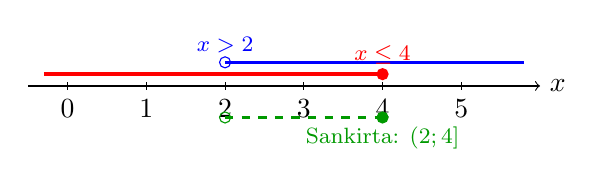
\begin{tikzpicture}
    \draw[->] (-0.5,0) -- (6,0) node[right] {$x$};
    \foreach \x/\lbl in {0/0,1/1,2/2,3/3,4/4,5/5}
        \draw (\x,0.05) -- (\x,-0.05) node[below] {$\lbl$};
    % Pirmoji nelygybė: x > 2
    \draw[blue, very thick] (2,0.3) -- (5.8,0.3);
    \draw[blue] (2,0.3) circle (2pt) node[above] {\footnotesize $x>2$};
    % Antroji nelygybė: x <= 4
    \draw[red, very thick] (-0.3,0.15) -- (4,0.15);
    \filldraw[red] (4,0.15) circle (2pt) node[above] {\footnotesize $x\leq4$};
    % Sankirta
    \draw[green!60!black, very thick, dashed] (2,-0.4) -- (4,-0.4);
    \draw[green!60!black] (2,-0.4) circle (2pt);
    \filldraw[green!60!black] (4,-0.4) circle (2pt) node[below] {\footnotesize Sankirta: $(2;4]$};
\end{tikzpicture}
\end{center}

\textbf{Atsakymas:} $x \in (2;\,4]$.
\end{example}

\begin{example}
Išspręskite nelygybių sistemą:
\[
\begin{cases}
    x + 5 > 3, \\
    3x - 2 < -8.
\end{cases}
\]

\textbf{Sprendimas:}

Pirmoji nelygybė: $x > -2$, t.y. $x \in (-2; +\infty)$.

Antroji nelygybė: $3x < -6 \implies x < -2$, t.y. $x \in (-\infty; -2)$.

Sankirta: $(-2; +\infty) \cap (-\infty; -2) = \emptyset$.

\textbf{Atsakymas:} Sistema neturi sprendinių.
\end{example}

\subsubsection{Sprendinių aibių užrašymas}

VBE egzamine svarbu mokėti sprendinių aibes užrašyti trimis būdais:

\begin{center}
\begin{tabular}{|l|l|l|}
\hline
\textbf{Nelygybė} & \textbf{Intervalų žymėjimas} & \textbf{Tiesė} \\
\hline
$x > a$ & $(a; +\infty)$ & atviras taškas, rodyklė dešinėn \\
$x \geq a$ & $[a; +\infty)$ & uždaras taškas, rodyklė dešinėn \\
$x < a$ & $(-\infty; a)$ & atviras taškas, rodyklė kairėn \\
$x \leq a$ & $(-\infty; a]$ & uždaras taškas, rodyklė kairėn \\
$a < x < b$ & $(a; b)$ & abu taškai atviri \\
$a \leq x \leq b$ & $[a; b]$ & abu taškai uždari \\
\hline
\end{tabular}
\end{center}

\subsubsection{VBE tipo uždaviniai}

\begin{exercise}
Raskite nelygybės $\dfrac{2x}{5} - \dfrac{x - 5}{4} \leq 0$ sprendinių intervalą.

\textbf{Sprendimas:} MBK$(5, 4) = 20$. Dauginame iš 20:
\[
8x - 5(x - 5) \leq 0 \implies 8x - 5x + 25 \leq 0 \implies 3x + 25 \leq 0 \implies x \leq -\frac{25}{3}.
\]

\textbf{Atsakymas:} $x \in \left(-\infty;\, -\dfrac{25}{3}\right]$.
\end{exercise}

\begin{exercise}
Raskite sveikuosius skaičius, tenkinančius sistemą:
\[
\begin{cases}
    2(x - 1) < x + 5, \\
    \dfrac{x + 4}{3} > 2.
\end{cases}
\]

\textbf{Sprendimas:}

Pirmoji nelygybė: $2x - 2 < x + 5 \implies x < 7$.

Antroji nelygybė: $x + 4 > 6 \implies x > 2$.

Sprendiniai: $x \in (2; 7)$.

Sveikieji skaičiai šiame intervale: $3, 4, 5, 6$.

\textbf{Atsakymas:} Sveikieji sprendiniai yra $3,\; 4,\; 5,\; 6$.
\end{exercise}

\section{Kvadratinės lygtys ir nelygybės}

\subsection{Kvadratinės lygtys}

\begin{definition}
\textbf{Kvadratinė lygtis} – tai lygtis, kurią galima užrašyti pavidalu:
\[
ax^2 + bx + c = 0,
\]
kur $a, b, c \in \mathbb{R}$, $a \neq 0$. Skaičiai $a$, $b$, $c$ vadinami lygties \textbf{koeficientais}: $a$ – vyriausiasis koeficientas, $b$ – antrojo nario koeficientas, $c$ – laisvasis narys.
\end{definition}

\begin{remark}
Jei $a = 0$, lygtis tampa tiesine. Todėl sąlyga $a \neq 0$ yra būtina, kad lygtis būtų kvadratinė.
\end{remark}

\subsubsection*{Diskriminantas}

Kvadratinės lygties $ax^2 + bx + c = 0$ sprendimui naudojama \textbf{diskriminanto} formulė:

\[
D = b^2 - 4ac.
\]

Diskriminantas lemia sprendinių skaičių ir pobūdį:

\begin{itemize}
    \item Jei $D > 0$ – lygtis turi \textbf{du skirtingus realiuosius sprendinius}.
    \item Jei $D = 0$ – lygtis turi \textbf{vieną (dvigubą) sprendinį}.
    \item Jei $D < 0$ – lygtis \textbf{neturi realiųjų sprendinių}.
\end{itemize}

\subsubsection*{Šaknų formulės}

Kai $D \geq 0$, kvadratinės lygties sprendiniai randami pagal formulę:

\[
x_{1,2} = \frac{-b \pm \sqrt{D}}{2a} = \frac{-b \pm \sqrt{b^2 - 4ac}}{2a}.
\]

Kai $D = 0$, gauname vieną sprendinį:
\[
x_0 = \frac{-b}{2a}.
\]

\begin{example}
Išspręskime lygtį $2x^2 - 5x + 3 = 0$.

Koeficientai: $a = 2$, $b = -5$, $c = 3$.

\[
D = (-5)^2 - 4 \cdot 2 \cdot 3 = 25 - 24 = 1 > 0.
\]

Kadangi $D > 0$, lygtis turi du skirtingus sprendinius:
\[
x_1 = \frac{5 + 1}{4} = \frac{6}{4} = \frac{3}{2}, \qquad x_2 = \frac{5 - 1}{4} = \frac{4}{4} = 1.
\]

\textit{Atsakymas:} $x_1 = \dfrac{3}{2}$, $x_2 = 1$.
\end{example}

\begin{example}
Išspręskime lygtį $x^2 - 4x + 4 = 0$.

\[
D = (-4)^2 - 4 \cdot 1 \cdot 4 = 16 - 16 = 0.
\]

\[
x_0 = \frac{4}{2} = 2.
\]

\textit{Atsakymas:} $x = 2$ (dviguba šaknis).
\end{example}

\begin{example}
Išspręskime lygtį $x^2 + x + 1 = 0$.

\[
D = 1 - 4 = -3 < 0.
\]

Lygtis neturi realiųjų sprendinių.
\end{example}

\subsubsection*{Specialiosios kvadratinių lygčių formos}

\paragraph{Redukuotoji kvadratinė lygtis.}
Kai $a = 1$, lygtis vadinama \textbf{redukuotąja}:
\[
x^2 + px + q = 0.
\]
Šaknų formulė supaprastėja:
\[
x_{1,2} = \frac{-p \pm \sqrt{p^2 - 4q}}{2}.
\]

\paragraph{Grynoji kvadratinė lygtis.}
Kai $b = 0$, lygtis vadinama \textbf{grynąja kvadratine lygtimi}:
\[
ax^2 + c = 0 \implies x^2 = -\frac{c}{a}.
\]
\begin{itemize}
    \item Jei $-\dfrac{c}{a} > 0$: $x_{1,2} = \pm\sqrt{-\dfrac{c}{a}}$.
    \item Jei $-\dfrac{c}{a} = 0$: $x = 0$.
    \item Jei $-\dfrac{c}{a} < 0$: realiųjų sprendinių nėra.
\end{itemize}

\paragraph{Nepilnoji kvadratinė lygtis.}
Kai $c = 0$, lygtis užrašoma:
\[
ax^2 + bx = 0 \implies x(ax + b) = 0.
\]
Sprendiniai: $x_1 = 0$ ir $x_2 = -\dfrac{b}{a}$.

\begin{tcolorbox}[title={VBE patarimas}]
Prieš taikydami diskriminanto formulę, visada patikrinkite, ar lygtis užrašyta standartine forma $ax^2 + bx + c = 0$. Perkeldami narius ir suprastindami sutaupysite laiko ir išvengsite klaidų.
\end{tcolorbox}

\subsubsection*{Kvadratinio trinario faktorizacija}

Jei kvadratinė lygtis $ax^2 + bx + c = 0$ turi sprendinius $x_1$ ir $x_2$, tai kvadratinis trinaris išskaidomas dauginamaisiais:
\[
ax^2 + bx + c = a(x - x_1)(x - x_2).
\]

\begin{example}
Lygtis $2x^2 - 5x + 3 = 0$ turi sprendinius $x_1 = \frac{3}{2}$ ir $x_2 = 1$, todėl:
\[
2x^2 - 5x + 3 = 2\!\left(x - \tfrac{3}{2}\right)(x - 1) = (2x - 3)(x - 1).
\]
\end{example}

\begin{exercise}
Išspręskite lygtis:
\begin{enumerate}[label=\alph*)]
    \item $3x^2 - 7x + 2 = 0$
    \item $x^2 - 6x + 9 = 0$
    \item $4x^2 + 1 = 0$
    \item $5x^2 - 20x = 0$
    \item $x^2 - 5x - 14 = 0$
\end{enumerate}
\end{exercise}

% -------------------------------------------------------------------
\subsection{Vieta ir koeficientų sąryšiai (Vijeto formulės)}
% -------------------------------------------------------------------

\begin{theorem}[Vijeto teorema]
Jei $x_1$ ir $x_2$ yra kvadratinės lygties $ax^2 + bx + c = 0$ ($a \neq 0$) sprendiniai, tai:
\[
x_1 + x_2 = -\frac{b}{a}, \qquad x_1 \cdot x_2 = \frac{c}{a}.
\]
\end{theorem}

\begin{proof}
Iš šaknų formulės:
\[
x_1 + x_2 = \frac{-b + \sqrt{D}}{2a} + \frac{-b - \sqrt{D}}{2a} = \frac{-2b}{2a} = -\frac{b}{a}.
\]
\[
x_1 \cdot x_2 = \frac{(-b + \sqrt{D})(-b - \sqrt{D})}{4a^2} = \frac{b^2 - D}{4a^2} = \frac{b^2 - (b^2 - 4ac)}{4a^2} = \frac{4ac}{4a^2} = \frac{c}{a}.
\]
\end{proof}

\subsubsection*{Vijeto formulės redukuotajai lygčiai}

Redukuotajai kvadratinei lygčiai $x^2 + px + q = 0$ Vijeto formulės įgauna ypač paprastą pavidalą:
\[
\boxed{x_1 + x_2 = -p, \qquad x_1 \cdot x_2 = q.}
\]

\begin{example}
Lygties $x^2 - 7x + 12 = 0$ sprendiniai $x_1, x_2$ tenkina:
\[
x_1 + x_2 = 7, \qquad x_1 \cdot x_2 = 12.
\]
Ieškome dviejų skaičių, kurių suma 7 ir sandauga 12: tai $3$ ir $4$.

Taigi $x_1 = 3$, $x_2 = 4$.
\end{example}

\subsubsection*{Atvirkštinė Vijeto teorema}

\begin{theorem}[Atvirkštinė Vijeto teorema]
Jei skaičiai $m$ ir $n$ tenkina sąlygas $m + n = -p$ ir $m \cdot n = q$, tai $m$ ir $n$ yra lygties $x^2 + px + q = 0$ sprendiniai.
\end{theorem}

Praktinis pritaikymas: norint sudaryti kvadratinę lygtį, kurios šaknys $x_1$ ir $x_2$, rašome:
\[
x^2 - (x_1 + x_2)x + x_1 x_2 = 0.
\]

\begin{example}
Sudarykime kvadratinę lygtį, kurios šaknys $x_1 = -3$ ir $x_2 = 5$.

\[
x_1 + x_2 = 2, \quad x_1 \cdot x_2 = -15.
\]

Lygtis: $x^2 - 2x - 15 = 0$.
\end{example}

\subsubsection*{Vijeto formulių taikymai}

Vijeto formulės leidžia rasti įvairias simetrinių išraiškų reikšmes nesprendžiant lygties:

\begin{itemize}
    \item $x_1^2 + x_2^2 = (x_1 + x_2)^2 - 2x_1 x_2$
    \item $x_1^2 - x_2^2 = (x_1 + x_2)(x_1 - x_2)$
    \item $(x_1 - x_2)^2 = (x_1 + x_2)^2 - 4x_1 x_2 = \dfrac{D}{a^2}$
    \item $x_1^3 + x_2^3 = (x_1 + x_2)^3 - 3x_1 x_2(x_1 + x_2)$
    \item $\dfrac{1}{x_1} + \dfrac{1}{x_2} = \dfrac{x_1 + x_2}{x_1 x_2}$ \quad (kai $x_1, x_2 \neq 0$)
\end{itemize}

\begin{example}
Lygties $2x^2 - 6x + 3 = 0$ šaknys $x_1, x_2$. Raskite $x_1^2 + x_2^2$.

Vijeto formulėmis: $x_1 + x_2 = 3$, $x_1 x_2 = \dfrac{3}{2}$.

\[
x_1^2 + x_2^2 = (x_1 + x_2)^2 - 2x_1 x_2 = 9 - 3 = 6.
\]
\end{example}

\begin{example}
Su kuriomis $k$ reikšmėmis lygties $x^2 + kx + (k+3) = 0$ šaknys lygios ir priešingų ženklų?

Vijeto formulėmis: $x_1 + x_2 = -k$ ir $x_1 x_2 = k + 3$.

Šaknys lygios ir priešingų ženklų, kai $x_1 + x_2 = 0$, t.~y.\ $-k = 0 \Rightarrow k = 0$.

Patikriname: kai $k = 0$, lygtis $x^2 + 3 = 0$ neturi realiųjų sprendinių. Taigi tokių $k$ nėra.
\end{example}

\begin{exercise}
\begin{enumerate}[label=\alph*)]
    \item Lygties $3x^2 + 12x - 6 = 0$ šaknys $x_1, x_2$. Raskite $x_1^2 + x_2^2$ ir $x_1^3 + x_2^3$.
    \item Sudarykite kvadratinę lygtį, kurios šaknys $x_1 = 1 + \sqrt{2}$, $x_2 = 1 - \sqrt{2}$.
    \item Su kuriomis $m$ reikšmėmis lygtis $x^2 - mx + (m+2) = 0$ turi dvi teigiamas šaknis?
    \item Raskite $\dfrac{1}{x_1} + \dfrac{1}{x_2}$, jei $x_1, x_2$ – lygties $5x^2 - 3x + 1 = 0$ šaknys.
\end{enumerate}
\end{exercise}

% -------------------------------------------------------------------
\subsection{Kvadratinės nelygybės}
% -------------------------------------------------------------------

\begin{definition}
\textbf{Kvadratinė nelygybė} – tai nelygybė pavidalo
\[
ax^2 + bx + c > 0 \quad \text{arba} \quad ax^2 + bx + c < 0 \quad (a \neq 0),
\]
taip pat su ženklais $\geq$ ir $\leq$.
\end{definition}

Kvadratinę nelygybę galima spręsti dviem pagrindiniais metodais: \textbf{grafiniu} ir \textbf{algebriniu (intervalų metodu)}.

\subsubsection*{Grafinis metodas}

Grafinis metodas remiasi parabolės $y = ax^2 + bx + c$ elgsena:

\begin{enumerate}
    \item Apskaičiuojame diskriminantą $D = b^2 - 4ac$.
    \item Randame parabolės ir $Ox$ ašies sankirtos taškus (jei jų yra).
    \item Nubraižome (arba įsivaizduojame) parabolę ir pagal nelygybės ženklą bei $a$ ženklą nustatome sprendinių aibę.
\end{enumerate}

\subsubsection*{Sprendinių aibė pagal $D$ ir $a$ ženklus}

\begin{center}
\begin{tabular}{|c|c|c|c|}
\hline
\textbf{Sąlyga} & \textbf{Nelygybė} & \textbf{Sprendinių aibė} \\
\hline
\multirow{2}{*}{$D > 0$, $a > 0$} & $ax^2+bx+c > 0$ & $(-\infty;\, x_1) \cup (x_2;\, +\infty)$ \\
                                   & $ax^2+bx+c < 0$ & $(x_1;\, x_2)$ \\
\hline
\multirow{2}{*}{$D > 0$, $a < 0$} & $ax^2+bx+c > 0$ & $(x_1;\, x_2)$ \\
                                   & $ax^2+bx+c < 0$ & $(-\infty;\, x_1) \cup (x_2;\, +\infty)$ \\
\hline
\multirow{2}{*}{$D = 0$, $a > 0$} & $ax^2+bx+c > 0$ & $(-\infty;\, x_0) \cup (x_0;\, +\infty)$ \\
                                   & $ax^2+bx+c < 0$ & $\emptyset$ \\
\hline
\multirow{2}{*}{$D = 0$, $a < 0$} & $ax^2+bx+c > 0$ & $\emptyset$ \\
                                   & $ax^2+bx+c < 0$ & $(-\infty;\, x_0) \cup (x_0;\, +\infty)$ \\
\hline
\multirow{2}{*}{$D < 0$, $a > 0$} & $ax^2+bx+c > 0$ & $\mathbb{R}$ \\
                                   & $ax^2+bx+c < 0$ & $\emptyset$ \\
\hline
\multirow{2}{*}{$D < 0$, $a < 0$} & $ax^2+bx+c > 0$ & $\emptyset$ \\
                                   & $ax^2+bx+c < 0$ & $\mathbb{R}$ \\
\hline
\end{tabular}
\end{center}

\noindent Čia $x_1 < x_2$ yra atitinkamos kvadratinės lygties šaknys, $x_0$ – dviguba šaknis.

\begin{remark}
Nelygybėse su $\geq$ arba $\leq$ šaknys $x_1$ ir $x_2$ \textbf{įtraukiamos} į sprendinių aibę (naudojami uždarieji intervalai).
\end{remark}

\subsubsection*{Algebrinis metodas (intervalų metodas)}

\begin{enumerate}
    \item Lygtį $ax^2 + bx + c = 0$ sprendžiame ir randame šaknis $x_1 \leq x_2$.
    \item Kvadratinį trinarį išskaidome dauginamaisiais:
    \[
    ax^2 + bx + c = a(x - x_1)(x - x_2).
    \]
    \item Skaičių tiesėje pažymime šaknis ir nustatome kiekvieno intervalo ženklą.
    \item Pagal nelygybės ženklą parenkame reikiamus intervalus.
\end{enumerate}

\begin{example}
Išspręskime nelygybę $x^2 - x - 6 < 0$.

\textbf{1 žingsnis.} Sprendžiame lygtį $x^2 - x - 6 = 0$:
\[
D = 1 + 24 = 25, \quad x_1 = \frac{1-5}{2} = -2, \quad x_2 = \frac{1+5}{2} = 3.
\]

\textbf{2 žingsnis.} Išskaidome dauginamaisiais:
\[
x^2 - x - 6 = (x + 2)(x - 3).
\]

\textbf{3 žingsnis.} Skaičių tiesė:

\[
\begin{array}{ccccccc}
& & x = -2 & & x = 3 & & \\
\hline
(x+2): & - & 0 & + & + & + & \\
(x-3): & - & - & - & 0 & + & \\
\hline
\text{sandauga}: & + & 0 & - & 0 & + &
\end{array}
\]

\textbf{4 žingsnis.} Mums reikia sandaugos $< 0$, t.~y.\ intervalo $(-2;\, 3)$.

\textit{Atsakymas:} $x \in (-2;\, 3)$.
\end{example}

\begin{example}
Išspręskime nelygybę $2x^2 + 3x + 5 > 0$.

\[
D = 9 - 40 = -31 < 0, \quad a = 2 > 0.
\]

Kadangi $D < 0$ ir $a > 0$, trinaris visoje $\mathbb{R}$ teigiamas.

\textit{Atsakymas:} $x \in \mathbb{R}$.
\end{example}

\begin{example}
Išspręskime nelygybę $-x^2 + 4x - 4 \geq 0$.

\[
D = 16 - 16 = 0, \quad x_0 = \frac{-4}{-2} = 2.
\]

Kadangi $a = -1 < 0$ ir $D = 0$, trinaris visur $\leq 0$, lygybė pasiekiama tik $x = 2$.

\textit{Atsakymas:} $x = 2$ (arba $x \in \{2\}$).
\end{example}

\subsubsection*{Sudėtingesnės nelygybės: kvadratinė nelygybė su parametru}

\begin{example}
Su kuriomis $k$ reikšmėmis nelygybė $kx^2 - 2x + 1 > 0$ tenkinama su visais $x \in \mathbb{R}$?

Tam reikia, kad parabolė $y = kx^2 - 2x + 1$ visuomet būtų virš $Ox$ ašies. Tam būtina:
\begin{itemize}
    \item $k > 0$ (parabolė atsiveria aukštyn),
    \item $D = 4 - 4k < 0 \Rightarrow k > 1$.
\end{itemize}

\textit{Atsakymas:} $k > 1$.
\end{example}

\begin{tcolorbox}[title={VBE patarimas}]
Spręsdami kvadratinę nelygybę, visada pradėkite nuo diskriminanto apskaičiavimo. Tai iš karto parodo, kiek šaknų turi atitinkama lygtis, ir padeda parinkti tinkamą sprendimo strategiją bei sprendinių aibės formą.
\end{tcolorbox}

\begin{exercise}
Išspręskite nelygybes:
\begin{enumerate}[label=\alph*)]
    \item $x^2 - 5x + 6 \leq 0$
    \item $2x^2 + x - 3 > 0$
    \item $-3x^2 + 12 \geq 0$
    \item $x^2 + 4x + 4 > 0$
    \item $x^2 - 2x + 5 < 0$
    \item $x^2 - (k+1)x + k \leq 0$ (spręskite pagal parametrą $k$)
\end{enumerate}
\end{exercise}

\section{Racionaliosios lygtys ir nelygybės}

Racionaliosios lygtys ir nelygybės yra tos, kuriose kintamasis pasirodo trupmenų skaitikliuose arba vardikliuose. Šiame skyriuje nagrinėsime jų sprendimo metodus, ypač svarbų \textbf{intervalų metodą}, kuris dažnai taikomas VBE užduotyse.

% -------------------------------------------------------
\subsection{Trupmeninės lygtys}

\begin{definition}
\textbf{Racionalioji (trupmeninė) lygtis} -- tai lygtis, kurioje yra bent viena trupmena su kintamuoju vardiklyje, t.~y. lygtis pavidalo
\[
    \frac{P(x)}{Q(x)} = R(x),
\]
kur $P(x)$, $Q(x)$, $R(x)$ -- daugiamio išraiškos, $Q(x) \neq 0$.
\end{definition}

\subsubsection*{Sprendimo algoritmas}

\begin{enumerate}
    \item \textbf{Rasti OBV (Bendras vardiklis).} Nustatyti visų lygties vardiklių bendrąjį vardiklį $D(x)$.
    \item \textbf{Padauginti abi puses iš $D(x)$.} Gauname lygtį be trupmenų.
    \item \textbf{Spręsti gautą lygtį} (tiesinę, kvadratinę ir t.~t.).
    \item \textbf{Patikrinti papildomąsias sąlygas (PS).} Kiekvienam gautam sprendiniui $x_0$ būtina patikrinti, ar $D(x_0) \neq 0$, t.~y. ar sprendinys nepatenka į trupmenų apibrėžimo srities draudimus. Sprendiniai, dėl kurių vardiklis lygus nuliui, \textbf{atmetami}.
\end{enumerate}

\begin{tcolorbox}[title={Dažna klaida!}, colback=red!5, colframe=red!60]
Daugiausia klaidų daroma pamiršus patikrinti papildomąsias sąlygas. Net jei skaičiai atrodo teisingi, visada patikrinkite, ar gauti sprendiniai neanuliuoja jokio vardiklio!
\end{tcolorbox}

\subsubsection*{Paprastas pavyzdys}

\begin{example}
Išspręsti lygtį:
\[
    \frac{x+3}{x-2} = 5.
\]

\textbf{Sprendimas.}

\textbf{PS:} $x \neq 2$.

Padauginame abi puses iš $(x - 2)$:
\[
    x + 3 = 5(x - 2).
\]
\[
    x + 3 = 5x - 10.
\]
\[
    3 + 10 = 5x - x \implies 4x = 13 \implies x = \frac{13}{4}.
\]
Tikriname PS: $\frac{13}{4} \neq 2$ -- \checkmark

\textbf{Atsakymas:} $x = \dfrac{13}{4}$.
\end{example}

\subsubsection*{Sudėtingesnis pavyzdys su keliais vardikliais}

\begin{example}
Išspręsti lygtį:
\[
    \frac{2}{x+1} + \frac{3}{x-1} = 1.
\]

\textbf{Sprendimas.}

\textbf{PS:} $x \neq -1$ ir $x \neq 1$.

Bendrasis vardiklis: $D(x) = (x+1)(x-1)$.

Padauginame abi puses iš $(x+1)(x-1)$:
\[
    2(x-1) + 3(x+1) = (x+1)(x-1).
\]
\[
    2x - 2 + 3x + 3 = x^2 - 1.
\]
\[
    5x + 1 = x^2 - 1.
\]
\[
    x^2 - 5x - 2 = 0.
\]

Diskriminantas: $\Delta = 25 + 8 = 33$.
\[
    x = \frac{5 \pm \sqrt{33}}{2}.
\]

Abu sprendiniai skirtingi nuo $\pm 1$, todėl abu tinka.

\textbf{Atsakymas:} $x = \dfrac{5 + \sqrt{33}}{2}$ arba $x = \dfrac{5 - \sqrt{33}}{2}$.
\end{example}

\subsubsection*{Atvejis, kai sprendinys atmetamas}

\begin{example}
Išspręsti lygtį:
\[
    \frac{x^2 - 4}{x - 2} = x + 2.
\]

\textbf{Sprendimas.}

\textbf{PS:} $x \neq 2$.

Pastebėkime, kad $x^2 - 4 = (x-2)(x+2)$, todėl:
\[
    \frac{(x-2)(x+2)}{x-2} = x+2 \implies x + 2 = x + 2.
\]

Ši lygybė teisinga visiems $x$, tačiau $x = 2$ atmetamas (PS).

\textbf{Atsakymas:} $x \in \mathbb{R} \setminus \{2\}$, t.~y. visi realieji skaičiai, išskyrus $x = 2$.
\end{example}

\begin{exercise}
Išspręskite lygtis:
\begin{enumerate}[label=\alph*)]
    \item $\dfrac{3x}{x+2} - \dfrac{6}{x-2} = \dfrac{x^2+12}{x^2-4}$
    \item $\dfrac{1}{x-3} + \dfrac{1}{x+3} = \dfrac{x}{x^2 - 9}$
    \item $\dfrac{x}{x-1} - \dfrac{2}{x+1} = \dfrac{5}{x^2-1}$
\end{enumerate}
\end{exercise}

% -------------------------------------------------------
\subsection{Racionaliosios nelygybės (intervalų metodas)}

\begin{definition}
\textbf{Racionalioji nelygybė} -- tai nelygybė pavidalo
\[
    \frac{P(x)}{Q(x)} > 0, \quad \frac{P(x)}{Q(x)} < 0, \quad \frac{P(x)}{Q(x)} \geq 0, \quad \frac{P(x)}{Q(x)} \leq 0,
\]
kur $P(x)$ ir $Q(x)$ -- daugiamiai. Reikia rasti visas $x$ reikšmes, kurių $Q(x) \neq 0$.
\end{definition}

\subsubsection*{Intervalų metodo algoritmas}

\begin{enumerate}
    \item \textbf{Pertvarkyti nelygybę į standartinį pavidalą.} Perkelti visus narius į vieną pusę taip, kad kitoje pusėje liktų $0$:
    \[
        \frac{P(x)}{Q(x)} \gtreqless 0.
    \]
    \item \textbf{Skaitiklį ir vardiklį išskaidyti dauginamaisiais.}
    \item \textbf{Rasti kritinius taškus.} Kritiniai taškai yra:
        \begin{itemize}
            \item \textbf{Skaitiklio šaknys} (čia išraiška lygi nuliui),
            \item \textbf{Vardiklio šaknys} (čia išraiška neapibrėžta -- šie taškai \emph{visada atmetami}).
        \end{itemize}
    \item \textbf{Pažymėti kritinius taškus ant skaičių tiesės} ir suskaidyti ją į intervalus.
    \item \textbf{Nustatyti išraiškos ženklą kiekviename intervale.} Galima naudoti \emph{ženklų lentelę} arba tikrinti su pasirinktu taško reikšme.
    \item \textbf{Surinkti atsakymą.} Atrinkti intervalus, kuriuose nelygybė tenkinama. Atkreipti dėmesį:
        \begin{itemize}
            \item Jei nelygybė \emph{griežta} ($>$ arba $<$), skaitiklio šaknys \textbf{neįtraukiamos}.
            \item Jei nelygybė \emph{nestrikte} ($\geq$ arba $\leq$), skaitiklio šaknys \textbf{įtraukiamos}.
            \item Vardiklio šaknys \textbf{niekada neįtraukiamos}.
        \end{itemize}
\end{enumerate}

\begin{tcolorbox}[title={Ženklų keitimosi taisyklė}, colback=blue!5, colframe=blue!50]
Kai $x$ pereina per paprastą šaknį (lygties $P(x)=0$ vienguba šaknis), išraiška \textbf{keičia ženklą}. Kai $x$ pereina per dvigubą (porinį) šaknį, ženklas \textbf{nesikeičia}.
\end{tcolorbox}

\subsubsection*{Paprastas pavyzdys}

\begin{example}
Išspręsti nelygybę:
\[
    \frac{x-1}{x+3} > 0.
\]

\textbf{Sprendimas.}

\textbf{1 žingsnis.} Nelygybė jau standartinio pavidalo.

\textbf{2 žingsnis.} Skaitiklis: $x - 1 = 0 \Rightarrow x = 1$. Vardiklis: $x + 3 = 0 \Rightarrow x = -3$ (atmetamas).

\textbf{3 žingsnis.} Kritiniai taškai: $x = -3$ ir $x = 1$. Jie padalija tiesę į 3 intervalus:
\[
    (-\infty;\, -3), \quad (-3;\, 1), \quad (1;\, +\infty).
\]

\textbf{4 žingsnis.} Ženklų lentelė:

\begin{center}
\begin{tabular}{c|ccccc}
$x$ & $(-\infty;-3)$ & $-3$ & $(-3;1)$ & $1$ & $(1;+\infty)$ \\
\hline
$x-1$ & $-$ & $-$ & $-$ & $0$ & $+$ \\
$x+3$ & $-$ & $0$ & $+$ & $+$ & $+$ \\
\hline
$\dfrac{x-1}{x+3}$ & $+$ & n.a. & $-$ & $0$ & $+$ \\
\end{tabular}
\end{center}

\textbf{5 žingsnis.} Mums reikia $> 0$, t.~y. „$+$" intervalai (be taško $x=1$, nes nelygybė griežta):

\textbf{Atsakymas:} $x \in (-\infty;\, -3) \cup (1;\, +\infty)$.
\end{example}

\subsubsection*{Sudėtingesnis pavyzdys}

\begin{example}
Išspręsti nelygybę:
\[
    \frac{x^2 - x - 6}{x^2 - 4} \leq 0.
\]

\textbf{Sprendimas.}

\textbf{1 žingsnis.} Skaidome dauginamaisiais:
\[
    x^2 - x - 6 = (x-3)(x+2), \quad x^2 - 4 = (x-2)(x+2).
\]

Taigi:
\[
    \frac{(x-3)(x+2)}{(x-2)(x+2)} \leq 0.
\]

Pastebime, kad $(x+2)$ yra abiejuose -- galime sutrumpinti, bet \textbf{tik tada}, kai $x \neq -2$:
\[
    \frac{x-3}{x-2} \leq 0, \quad x \neq -2.
\]

\textbf{2 žingsnis.} Kritiniai taškai:
\begin{itemize}
    \item Skaitiklis: $x = 3$ (įtraukiamas, nes $\leq$),
    \item Vardiklis: $x = 2$ (niekada neįtraukiamas),
    \item Papildomai atmesta: $x = -2$ (dėl sutrumpinimo).
\end{itemize}

\textbf{3 žingsnis.} Skaičių tiesė su intervalais: $(-\infty;\,2),\;(2;\,3],\;(3;\,+\infty)$.

\begin{center}
\begin{tabular}{c|ccccc}
$x$ & $(-\infty;2)$ & $2$ & $(2;3)$ & $3$ & $(3;+\infty)$ \\
\hline
$x-3$ & $-$ & $-$ & $-$ & $0$ & $+$ \\
$x-2$ & $-$ & $0$ & $+$ & $+$ & $+$ \\
\hline
$\dfrac{x-3}{x-2}$ & $+$ & n.a. & $-$ & $0$ & $+$ \\
\end{tabular}
\end{center}

Mums reikia $\leq 0$ (neigiamų ir lygių nuliui):

\textbf{Atsakymas:} $x \in (2;\, 3]$, nes $x = -2$ atmetamas ir $x = 2$ atmestinas (vardiklis).
\end{example}

\subsubsection*{Nelygybė su persitvarkymu}

\begin{example}
Išspręsti nelygybę:
\[
    \frac{2}{x-1} \geq 3.
\]

\textbf{Sprendimas.}

\textbf{1 žingsnis.} Perkeliame $3$ į kairę:
\[
    \frac{2}{x-1} - 3 \geq 0.
\]

Suvedame į bendrą trupmeną:
\[
    \frac{2 - 3(x-1)}{x-1} \geq 0 \implies \frac{2 - 3x + 3}{x-1} \geq 0 \implies \frac{5 - 3x}{x-1} \geq 0.
\]

\textbf{2 žingsnis.} Kritiniai taškai:
\begin{itemize}
    \item Skaitiklis: $5 - 3x = 0 \Rightarrow x = \dfrac{5}{3}$ (įtraukiamas, nes $\geq$),
    \item Vardiklis: $x = 1$ (neįtraukiamas).
\end{itemize}

\textbf{3 žingsnis.} Ženklų lentelė:

\begin{center}
\begin{tabular}{c|ccccc}
$x$ & $(-\infty;1)$ & $1$ & $\left(1;\frac{5}{3}\right)$ & $\frac{5}{3}$ & $\left(\frac{5}{3};+\infty\right)$ \\
\hline
$5-3x$ & $+$ & $+$ & $+$ & $0$ & $-$ \\
$x-1$ & $-$ & $0$ & $+$ & $+$ & $+$ \\
\hline
$\dfrac{5-3x}{x-1}$ & $-$ & n.a. & $+$ & $0$ & $-$ \\
\end{tabular}
\end{center}

Mums reikia $\geq 0$:

\textbf{Atsakymas:} $x \in \left(1;\, \dfrac{5}{3}\right]$.
\end{example}

\begin{remark}
\textbf{Svarbu!} Negalima dauginti nelygybės iš $x-1$ tiesiogiai, nes nežinome, ar šis daugiklis teigiamas, ar neigiamas. Todėl visuomet naudojame pertvarkymą su nuliu, o ne tiesiogiai dauginame iš vardiklio.
\end{remark}

\begin{exercise}
Išspręskite nelygybes intervalų metodu:
\begin{enumerate}[label=\alph*)]
    \item $\dfrac{x+4}{x-3} < 0$
    \item $\dfrac{x^2 - 5x + 6}{x+1} \geq 0$
    \item $\dfrac{3}{x+2} \leq 1$
    \item $\dfrac{x^2 - 1}{x^2 - 9} > 0$
    \item $\dfrac{(x-2)(x+5)}{(x-1)(x+3)} \leq 0$
\end{enumerate}
\end{exercise}

\begin{tcolorbox}[title={VBE patarimai}, colback=green!5, colframe=green!60]
\begin{itemize}
    \item Visada rašykite \textbf{papildomąsias sąlygas} (PS) prieš pradedant spręsti trupmeninę lygtį.
    \item Intervalų metode \textbf{niekada} nemėginkite dauginti nelygybės iš kintamojo reiškinio -- tai pakeis nelygybės kryptį, jei reiškinys neigiamas.
    \item Atsakymą rašykite \textbf{intervalo žymėjimu} arba naudodami nelygybių sistemas.
    \item Dvigubos šaknys (\emph{porinis kartotingumas}) \textbf{nekeičia} ženklo -- atidžiai žiūrėkite į dauginamaisiais išskaidytą išraišką.
\end{itemize}
\end{tcolorbox}

\section{Eksponentinės lygtys ir nelygybės}

Eksponentinė lygtis – tai lygtis, kurioje nežinomasis yra laipsnio rodiklyje (eksponentėje). 
Bendra forma: $a^{f(x)} = b$, kur $a > 0$, $a \neq 1$.

\subsection{Pagrindiniai sprendimo būdai}

\begin{definition}
\textbf{Eksponentinė lygtis} – lygtis, kurioje nežinomasis $x$ yra laipsnio rodiklyje. 
Bendroji forma: $a^{f(x)} = a^{g(x)}$, kur $a > 0$, $a \neq 1$, arba $a^{f(x)} = b$.
\end{definition}

Pagrindinė savybė, kuria remiamasi sprendžiant eksponentines lygtis, yra eksponentinės 
funkcijos injektyvumas (vienas-su-vienu):

\begin{theorem}[Eksponentinės lygties pagrindinis principas]
Jei $a > 0$, $a \neq 1$, tai
\[
a^{f(x)} = a^{g(x)} \iff f(x) = g(x).
\]
\end{theorem}

\subsubsection*{I būdas: Vienodinimas pagrindo}

Šis būdas taikomas, kai abi lygties pusės gali būti išreikštos to paties pagrindo laipsniais.

\textbf{Algoritmas:}
\begin{enumerate}
    \item Išreikšti abi lygties puses to paties pagrindo $a$ laipsniais.
    \item Sulyginti rodiklius: $f(x) = g(x)$.
    \item Išspręsti gautą lygtį.
\end{enumerate}

\begin{example}
Išspręsti lygtį $4^{x} = 8$.

\textbf{Sprendimas:}
\[
4^x = 8 \implies (2^2)^x = 2^3 \implies 2^{2x} = 2^3 \implies 2x = 3 \implies x = \frac{3}{2}.
\]
\textbf{Atsakymas:} $x = \dfrac{3}{2}$.
\end{example}

\begin{example}
Išspręsti lygtį $9^{x-1} = 27^{x+2}$.

\textbf{Sprendimas:}
\[
(3^2)^{x-1} = (3^3)^{x+2} \implies 3^{2(x-1)} = 3^{3(x+2)}
\]
\[
2(x-1) = 3(x+2) \implies 2x - 2 = 3x + 6 \implies x = -8.
\]
\textbf{Atsakymas:} $x = -8$.
\end{example}

\subsubsection*{II būdas: Kintamojo keitimas (pakeitimas)}

Šis būdas taikomas, kai lygtis yra kvadratinė eksponentės atžvilgiu arba gali būti 
redukuota į algebrinę lygtį.

\textbf{Algoritmas:}
\begin{enumerate}
    \item Įvesti pakeitimą $t = a^x$ (kur $t > 0$).
    \item Išspręsti gautą algebrinę lygtį $t$ atžvilgiu.
    \item Grąžinti pakeitimą ir išspręsti eksponentinę lygtį $x$ atžvilgiu.
    \item Patikrinti, ar $t > 0$ (jei $t \leq 0$ – šaknis atmetama).
\end{enumerate}

\begin{example}
Išspręsti lygtį $4^{x} - 3 \cdot 2^{x} - 4 = 0$.

\textbf{Sprendimas:} Pastebime, kad $4^x = (2^2)^x = (2^x)^2$.

Darome pakeitimą $t = 2^x$, $t > 0$:
\[
t^2 - 3t - 4 = 0.
\]
Diskriminantas: $D = 9 + 16 = 25$.
\[
t_1 = \frac{3+5}{2} = 4, \quad t_2 = \frac{3-5}{2} = -1.
\]
Kadangi $t > 0$, tai $t_2 = -1$ atmetame.

Iš $t_1 = 4$:
\[
2^x = 4 = 2^2 \implies x = 2.
\]
\textbf{Atsakymas:} $x = 2$.
\end{example}

\begin{example}
Išspręsti lygtį $3^{2x} - 10 \cdot 3^{x} + 9 = 0$.

\textbf{Sprendimas:} Darome pakeitimą $t = 3^x$, $t > 0$:
\[
t^2 - 10t + 9 = 0 \implies (t-1)(t-9) = 0.
\]
\[
t_1 = 1, \quad t_2 = 9.
\]
\begin{itemize}
    \item Jei $3^x = 1 = 3^0$, tai $x = 0$.
    \item Jei $3^x = 9 = 3^2$, tai $x = 2$.
\end{itemize}
\textbf{Atsakymas:} $x \in \{0;\, 2\}$.
\end{example}

\subsubsection*{III būdas: Logaritmavimas}

Šis būdas taikomas, kai lygties pusių negalima išreikšti to paties pagrindo laipsniais, 
arba kai tai patogu.

\begin{theorem}
Jei $a^{f(x)} = b$, kur $b > 0$, tai
\[
f(x) = \log_a b.
\]
Ekvivalenčiai, logaritmuojant abi puses:
\[
f(x) \cdot \ln a = \ln b \implies f(x) = \frac{\ln b}{\ln a}.
\]
\end{theorem}

\begin{example}
Išspręsti lygtį $5^{x} = 7$.

\textbf{Sprendimas:}
\[
5^x = 7 \implies x = \log_5 7 = \frac{\ln 7}{\ln 5} \approx \frac{1{,}9459}{1{,}6094} \approx 1{,}21.
\]
\textbf{Atsakymas:} $x = \log_5 7$.
\end{example}

\begin{example}
Išspręsti lygtį $2^{x+1} = 3^{x-1}$.

\textbf{Sprendimas:} Logaritmuojame abi puses (natūraliuoju logaritmu):
\[
(x+1)\ln 2 = (x-1)\ln 3.
\]
\[
x \ln 2 + \ln 2 = x \ln 3 - \ln 3.
\]
\[
x(\ln 2 - \ln 3) = -\ln 3 - \ln 2.
\]
\[
x = \frac{-\ln 3 - \ln 2}{\ln 2 - \ln 3} = \frac{\ln 6}{\ln 3 - \ln 2} = \frac{\ln 6}{\ln(3/2)}.
\]
\textbf{Atsakymas:} $x = \dfrac{\ln 6}{\ln(3/2)} = \log_{3/2} 6$.
\end{example}

\begin{remark}
Pasirenkant logaritmavimo pagrindą svarbu atsiminti:
\begin{itemize}
    \item Jei lygtyje yra $10^x$ – patogu logaritmuoti dešimtiniu logaritmu ($\lg$).
    \item Jei lygtyje yra $e^x$ – patogu logaritmuoti natūraliuoju logaritmu ($\ln$).
    \item Kitais atvejais galima naudoti bet kurį logaritmą.
\end{itemize}
\end{remark}

\subsubsection*{Sudėtingesnės lygtys ir sistemos}

\begin{example}
Išspręsti lygčių sistemą:
\[
\begin{cases}
2^x \cdot 3^y = 72, \\
4^x \cdot 9^y = 5184.
\end{cases}
\]

\textbf{Sprendimas:} Pastebime, kad $72 = 8 \cdot 9 = 2^3 \cdot 3^2$ ir 
$5184 = 72^2 = 2^6 \cdot 3^4$. Antra lygtis yra pirmosios kvadratas, tačiau 
patikrinkime: $4^x \cdot 9^y = (2^2)^x \cdot (3^2)^y = 2^{2x} \cdot 3^{2y}$.

Darome pakeitimą $u = 2^x$, $v = 3^y$ (kur $u, v > 0$):
\[
\begin{cases}
u \cdot v = 72, \\
u^2 \cdot v^2 = 5184.
\end{cases}
\]
Antroji lygtis: $(uv)^2 = 5184 = 72^2$, taigi $uv = 72$ (nes $u,v>0$). 

Sistema yra suderinta. Papildomai iš pirmosios lygties: $2^x \cdot 3^y = 2^3 \cdot 3^2$.

Lyginant dėmenis (laikant $x, y$ sveikaisiais sprendiniais):
$x = 3$, $y = 2$.

\textbf{Atsakymas:} $x = 3$, $y = 2$.
\end{example}

% -------------------------------------------------------
\subsection{Eksponentinės nelygybės}
% -------------------------------------------------------

\begin{definition}
\textbf{Eksponentinė nelygybė} – nelygybė, kurioje nežinomasis yra laipsnio rodiklyje. 
Bendroji forma: $a^{f(x)} \gtrless a^{g(x)}$ arba $a^{f(x)} \gtrless b$.
\end{definition}

Eksponentinės nelygybės sprendimas esminiu būdu priklauso nuo pagrindo $a$ dydžio. 
Tai lemia, ar funkcija $a^x$ yra didėjanti, ar mažėjanti.

\begin{theorem}[Eksponentinės nelygybės sprendimo principas]
Tegu $a > 0$, $a \neq 1$. Tada:
\begin{enumerate}
    \item Jei $a > 1$ (funkcija \textbf{didėjanti}):
    \[
    a^{f(x)} > a^{g(x)} \iff f(x) > g(x).
    \]
    \item Jei $0 < a < 1$ (funkcija \textbf{mažėjanti}):
    \[
    a^{f(x)} > a^{g(x)} \iff f(x) < g(x).
    \]
\end{enumerate}
Kitaip tariant, kai $0 < a < 1$, nelygybės ženklas \textbf{keičiasi į priešingą}.
\end{theorem}

\begin{tcolorbox}[title={Atminties lentelė: nelygybės ženklas}, colback=blue!5!white, colframe=blue!60!black]
\begin{center}
\begin{tabular}{|c|c|c|}
\hline
\textbf{Pagrindas} & \textbf{Funkcija} & \textbf{Nelygybės ženklas} \\
\hline
$a > 1$ & Didėjanti & Nesikeičia \\
$0 < a < 1$ & Mažėjanti & \textbf{Keičiasi į priešingą} \\
\hline
\end{tabular}
\end{center}
\end{tcolorbox}

\subsubsection*{Paprastos eksponentinės nelygybės}

\begin{example}
Išspręsti nelygybę $3^{2x-1} > 27$.

\textbf{Sprendimas:} Pagrindas $a = 3 > 1$, tai funkcija didėjanti.
\[
3^{2x-1} > 3^3 \implies 2x - 1 > 3 \implies 2x > 4 \implies x > 2.
\]
\textbf{Atsakymas:} $x \in (2;\, +\infty)$.
\end{example}

\begin{example}
Išspręsti nelygybę $\left(\dfrac{1}{5}\right)^{x+2} \leq 25$.

\textbf{Sprendimas:} Pagrindas $a = \dfrac{1}{5} < 1$, tai funkcija mažėjanti.
\[
25 = \frac{1}{5^{-2}} = \left(\frac{1}{5}\right)^{-2}.
\]
\[
\left(\frac{1}{5}\right)^{x+2} \leq \left(\frac{1}{5}\right)^{-2} \implies x + 2 \geq -2 
\implies x \geq -4.
\]
(Nelygybės ženklas pasikeitė, nes $0 < a < 1$.)

\textbf{Atsakymas:} $x \in [-4;\, +\infty)$.
\end{example}

\begin{example}
Išspręsti nelygybę $\left(0{,}2\right)^{3x-1} > \left(0{,}04\right)^{x+1}$.

\textbf{Sprendimas:} Pastebime, kad $0{,}04 = (0{,}2)^2$, taigi:
\[
(0{,}2)^{3x-1} > (0{,}2)^{2(x+1)}.
\]
Pagrindas $a = 0{,}2 < 1$, tai ženklas keičiasi:
\[
3x - 1 < 2(x+1) \implies 3x - 1 < 2x + 2 \implies x < 3.
\]
\textbf{Atsakymas:} $x \in (-\infty;\, 3)$.
\end{example}

\subsubsection*{Eksponentinės nelygybės su kintamojo pakeitimu}

Sudėtingesnėse nelygybėse, analogiškai lygčių sprendimui, taikomas kintamojo keitimas.

\begin{example}
Išspręsti nelygybę $4^x - 5 \cdot 2^x + 4 \leq 0$.

\textbf{Sprendimas:} Darome pakeitimą $t = 2^x$, $t > 0$. Kadangi $4^x = t^2$:
\[
t^2 - 5t + 4 \leq 0.
\]
Randame šaknis: $t^2 - 5t + 4 = (t-1)(t-4) = 0 \implies t_1 = 1,\; t_2 = 4$.

Nelygybė $(t-1)(t-4) \leq 0$ tenkinama, kai $1 \leq t \leq 4$.

Grąžiname pakeitimą ($t = 2^x$, pagrindas $2 > 1$):
\[
1 \leq 2^x \leq 4 \implies 2^0 \leq 2^x \leq 2^2 \implies 0 \leq x \leq 2.
\]
\textbf{Atsakymas:} $x \in [0;\, 2]$.
\end{example}

\begin{example}
Išspręsti nelygybę $9^x - 4 \cdot 3^{x+1} + 27 > 0$.

\textbf{Sprendimas:} Darome pakeitimą $t = 3^x$, $t > 0$. Kadangi $9^x = t^2$ ir 
$3^{x+1} = 3 \cdot 3^x = 3t$:
\[
t^2 - 12t + 27 > 0.
\]
Randame šaknis: diskriminantas $D = 144 - 108 = 36$, 
$t_1 = \dfrac{12-6}{2} = 3$, $t_2 = \dfrac{12+6}{2} = 9$.

Nelygybė $t^2 - 12t + 27 > 0$ tenkinama, kai $t < 3$ arba $t > 9$.

Grąžiname pakeitimą ($t = 3^x > 0$, pagrindas $3 > 1$):
\begin{itemize}
    \item $3^x < 3 \implies x < 1$.
    \item $3^x > 9 = 3^2 \implies x > 2$.
\end{itemize}
\textbf{Atsakymas:} $x \in (-\infty;\, 1) \cup (2;\, +\infty)$.
\end{example}

\subsubsection*{Nelygybių sistemos}

\begin{example}
Išspręsti nelygybių sistemą:
\[
\begin{cases}
2^{x} > \dfrac{1}{4}, \\[6pt]
\left(\dfrac{1}{3}\right)^{x} < 9.
\end{cases}
\]

\textbf{Sprendimas:}

\textit{Pirmoji nelygybė:} $2^x > 2^{-2}$, pagrindas $2 > 1$:
\[
x > -2.
\]

\textit{Antroji nelygybė:} $\left(\dfrac{1}{3}\right)^x < 3^2 = \left(\dfrac{1}{3}\right)^{-2}$, 
pagrindas $\dfrac{1}{3} < 1$, ženklas keičiasi:
\[
x > -2.
\]

Abiejų nelygybių sprendinių sankirtą gauname:
\[
x > -2 \quad \text{ir} \quad x > -2 \implies x > -2.
\]
\textbf{Atsakymas:} $x \in (-2;\, +\infty)$.
\end{example}

\begin{remark}
Sprendžiant eksponentines nelygybes svarbu:
\begin{itemize}
    \item Visada nustatyti pagrindo $a$ reikšmę ($a > 1$ ar $0 < a < 1$).
    \item Vienodinant pagrindu, perkelti visus narius į vieną pusę arba naudoti kintamojo 
    pakeitimą.
    \item Taikant kintamojo pakeitimą $t = a^x$, visada atsiminti, kad $t > 0$.
    \item Galutinį atsakymą užrašyti intervalo forma.
\end{itemize}
\end{remark}

\subsubsection*{VBE tipo uždaviniai}

\begin{exercise}
Išspręskite eksponentines lygtis:
\begin{enumerate}[label=\alph*)]
    \item $2^{3x-1} = 16$
    \item $5^{x^2 - 4} = 1$
    \item $3^{2x} - 10 \cdot 3^x + 9 = 0$
    \item $6^x = 10$
    \item $2^{x+3} = 5^{x-1}$
\end{enumerate}
\end{exercise}

\begin{exercise}
Išspręskite eksponentines nelygybes:
\begin{enumerate}[label=\alph*)]
    \item $\left(\dfrac{1}{2}\right)^{x-3} \geq 8$
    \item $5^{2x-1} < 125$
    \item $4^x - 3 \cdot 2^{x+1} + 8 \leq 0$
    \item $\left(0{,}3\right)^{x^2-1} \geq \left(0{,}3\right)^{2x}$
\end{enumerate}
\end{exercise}

\begin{exercise}[VBE formato]
Įmonės pelnas (tūkst. eurų) $t$ metų po įkūrimo aprašomas formule 
$P(t) = 5 \cdot 1{,}2^t$.
\begin{enumerate}[label=\alph*)]
    \item Raskite, po kiek metų pelnas viršys 25 tūkst. eurų.
    \item Kada pelnas bus didesnis nei 50 tūkst. eurų?
\end{enumerate}
\textit{Sprendimas (a):} $5 \cdot 1{,}2^t > 25 \implies 1{,}2^t > 5 \implies 
t > \log_{1{,}2} 5 = \dfrac{\ln 5}{\ln 1{,}2} \approx \dfrac{1{,}609}{0{,}182} \approx 8{,}8.$

Vadinasi, po $9$ metų.
\end{exercise}

\section{Logaritminės lygtys ir nelygybės}

\subsection{Pagrindiniai sprendimo būdai}

Logaritminė lygtis yra lygtis, kurioje nežinomasis yra logaritmo argumente arba pagrinde. Sprendžiant logaritmines lygtis naudojami keli pagrindiniai metodai.

\begin{tcolorbox}[title={Svarbiausios logaritmų savybės (priminimai)}]
Tegu $a > 0,\ a \neq 1,\ b > 0,\ c > 0$. Tada:
\begin{align}
\log_a(b \cdot c) &= \log_a b + \log_a c \\
\log_a\!\left(\frac{b}{c}\right) &= \log_a b - \log_a c \\
\log_a b^n &= n \cdot \log_a b,\quad n \in \mathbb{R} \\
\log_a b &= \frac{\log_c b}{\log_c a} \quad \text{(pagrindo keitimas)} \\
a^{\log_a b} &= b
\end{align}
\end{tcolorbox}

\subsubsection*{1 metodas: Tiesioginis taikymas pagal apibrėžimą}

Paprasčiausia logaritminė lygtis yra pavidalo $\log_a f(x) = b$. Ji ekvivalenti sąlygai:
\[
f(x) = a^b, \quad \text{kai } f(x) > 0,\ a > 0,\ a \neq 1.
\]

\begin{example}
Išspręskime lygtį $\log_3(2x - 1) = 3$.

\textbf{Sprendimas:}
\begin{align*}
\log_3(2x - 1) &= 3 \\
2x - 1 &= 3^3 = 27 \\
2x &= 28 \\
x &= 14.
\end{align*}
\textbf{Patikrinimas:} $\log_3(2 \cdot 14 - 1) = \log_3 27 = 3$ \checkmark

\textbf{Atsakymas:} $x = 14$.
\end{example}

\begin{remark}
Visada reikia patikrinti, ar logaritmo argumentas yra teigiamas. Jei sprendinys šios sąlygos netenkina, jis atmetamas.
\end{remark}

\subsubsection*{2 metodas: Logaritmų vienalytiškumo savybė}

Jei $\log_a f(x) = \log_a g(x)$, tuomet $f(x) = g(x)$ (su sąlyga, kad $f(x) > 0$ ir $g(x) > 0$).

\begin{example}
Išspręskime lygtį $\log_5(3x + 1) = \log_5(x + 7)$.

\textbf{Sprendimas:}
\begin{align*}
3x + 1 &= x + 7 \\
2x &= 6 \\
x &= 3.
\end{align*}
\textbf{Patikrinimas:} $3 \cdot 3 + 1 = 10 > 0$, $3 + 7 = 10 > 0$ \checkmark

\textbf{Atsakymas:} $x = 3$.
\end{example}

\subsubsection*{3 metodas: Logaritmų savybių naudojimas (sujungimas)}

Kai lygtyje yra logaritmų suma arba skirtumas, naudojamos savybės, kad logaritmai sujungiami į vieną.

\begin{example}
Išspręskime lygtį $\log_2 x + \log_2(x - 2) = 3$.

\textbf{Sprendimas:}
\begin{align*}
\log_2\bigl(x(x-2)\bigr) &= 3 \\
x(x - 2) &= 2^3 = 8 \\
x^2 - 2x - 8 &= 0 \\
(x - 4)(x + 2) &= 0 \\
x_1 = 4,&\quad x_2 = -2.
\end{align*}
\textbf{Patikrinimas:}
\begin{itemize}
    \item $x_1 = 4$: $\log_2 4 + \log_2 2 = 2 + 1 = 3$ \checkmark
    \item $x_2 = -2$: $\log_2(-2)$ — nėra apibrėžtas, \textbf{atmetamas}.
\end{itemize}

\textbf{Atsakymas:} $x = 4$.
\end{example}

\subsubsection*{4 metodas: Keitinys (substitucija)}

Kai lygtyje kartojasi ta pati logaritminė išraiška, įvedamas keitinys $t = \log_a f(x)$. Taip lygtis redukuojama į algebrinę (dažniausiai kvadratinę).

\begin{example}
Išspręskime lygtį $\lg^2 x - 3\lg x + 2 = 0$.

\textbf{Sprendimas.} Įvedame keitinį $t = \lg x$:
\begin{align*}
t^2 - 3t + 2 &= 0 \\
(t - 1)(t - 2) &= 0 \\
t_1 = 1, &\quad t_2 = 2.
\end{align*}
Grįžtame prie kintamojo $x$:
\begin{align*}
\lg x &= 1 \implies x_1 = 10, \\
\lg x &= 2 \implies x_2 = 100.
\end{align*}

\textbf{Atsakymas:} $x_1 = 10,\ x_2 = 100$.
\end{example}

\begin{example}
Išspręskime lygtį $\log_2 x + \log_x 2 = 2$.

\textbf{Sprendimas.} Pasinaudojame pagrindo keitimo formule: $\log_x 2 = \dfrac{1}{\log_2 x}$.

Įvedame keitinį $t = \log_2 x$ ($t \neq 0$, $x > 0$, $x \neq 1$):
\[
t + \frac{1}{t} = 2 \implies t^2 - 2t + 1 = 0 \implies (t-1)^2 = 0 \implies t = 1.
\]
\[
\log_2 x = 1 \implies x = 2.
\]

\textbf{Atsakymas:} $x = 2$.
\end{example}

\subsubsection*{5 metodas: Pagrindo keitimas}

Kai logaritmų pagrindai skirtingi, naudojama pagrindo keitimo formulė, kad visi logaritmai turėtų vienodą pagrindą:
\[
\log_a b = \frac{\ln b}{\ln a} = \frac{\lg b}{\lg a}.
\]

\begin{example}
Išspręskime lygtį $\log_4 x = \log_2 3$.

\textbf{Sprendimas:}
\[
\log_4 x = \log_2 3 \implies \frac{\log_2 x}{\log_2 4} = \log_2 3 \implies \frac{\log_2 x}{2} = \log_2 3 \implies \log_2 x = \log_2 9 \implies x = 9.
\]

\textbf{Atsakymas:} $x = 9$.
\end{example}

\begin{tcolorbox}[title={Logaritminių lygčių sprendimo algoritmas}]
\begin{enumerate}
    \item Nustatyti \textbf{egzistavimo sąlygas} (argumentai $> 0$, pagrindas $> 0$ ir $\neq 1$).
    \item Naudoti logaritmų savybes, kad lygtis būtų supaprastinta.
    \item Spręsti gautą algebrinę arba logaritminę lygtį.
    \item \textbf{Patikrinti sprendinius} ir atmesti netinkamus.
\end{enumerate}
\end{tcolorbox}

% ─────────────────────────────────────────────────────────────────
\subsection{Logaritminės nelygybės}

Logaritminė nelygybė — tai nelygybė, kurioje nežinomasis yra logaritmo argumente. Logaritminės nelygybės sprendiniai priklauso nuo logaritmo \textbf{pagrindo}.

\begin{tcolorbox}[title={Pagrindinis principas}]
Tegu $a > 0,\ a \neq 1$, ir $f(x),\, g(x) > 0$. Tada:
\[
\log_a f(x) \lessgtr \log_a g(x) \iff
\begin{cases}
f(x) \lessgtr g(x), & \text{jei } a > 1, \\
f(x) \gtrless g(x), & \text{jei } 0 < a < 1.
\end{cases}
\]
\textbf{Svarbu:} Kai $0 < a < 1$, nelygybes ženklas \textbf{apsiverčia}!
\end{tcolorbox}

\subsubsection*{Paprastos logaritminės nelygybės}

\begin{example}
Išspręskime nelygybę $\log_3(x - 1) > 2$.

\textbf{Sprendimas.} Pagrindas $a = 3 > 1$, tad:
\[
x - 1 > 3^2 = 9 \implies x > 10.
\]
Egzistavimo sąlyga: $x - 1 > 0 \implies x > 1$. Ji tenkinoma, kai $x > 10$.

\textbf{Atsakymas:} $x \in (10, +\infty)$.
\end{example}

\begin{example}
Išspręskime nelygybę $\log_{1/2}(x + 3) \geq -1$.

\textbf{Sprendimas.} Pagrindas $a = \tfrac{1}{2} < 1$, tad nelygybes ženklas \textbf{apsiverčia}:
\[
x + 3 \leq \left(\frac{1}{2}\right)^{-1} = 2 \implies x \leq -1.
\]
Egzistavimo sąlyga: $x + 3 > 0 \implies x > -3$.

Sprendinys: $-3 < x \leq -1$.

\textbf{Atsakymas:} $x \in (-3, -1]$.
\end{example}

\subsubsection*{Nelygybės su logaritmų savybėmis}

\begin{example}
Išspręskime nelygybę $\log_2 x + \log_2(x - 3) > 2$.

\textbf{Sprendimas.}

\textit{Egzistavimo sąlygos:} $x > 0$ ir $x - 3 > 0 \implies x > 3$.

Sujungiame logaritmus:
\[
\log_2\bigl(x(x-3)\bigr) > 2 \implies x(x-3) > 2^2 = 4 \implies x^2 - 3x - 4 > 0.
\]
Kvadratinės nelygybės sprendimas:
\[
(x - 4)(x + 1) > 0 \implies x < -1 \text{ arba } x > 4.
\]
Atsižvelgiant į egzistavimo sąlygą $x > 3$, gauname $x > 4$.

\textbf{Atsakymas:} $x \in (4, +\infty)$.
\end{example}

\subsubsection*{Nelygybės su keitiniu}

\begin{example}
Išspręskime nelygybę $\lg^2 x - \lg x - 2 < 0$.

\textbf{Sprendimas.} Įvedame keitinį $t = \lg x$ (čia $x > 0$):
\[
t^2 - t - 2 < 0 \implies (t - 2)(t + 1) < 0 \implies -1 < t < 2.
\]
Grąžiname keitinį:
\[
-1 < \lg x < 2 \implies 10^{-1} < x < 10^2 \implies \frac{1}{10} < x < 100.
\]

\textbf{Atsakymas:} $x \in \left(\dfrac{1}{10},\ 100\right)$.
\end{example}

\begin{example}
Išspręskime nelygybę $\log_{\frac{1}{3}}(x^2 - 5x + 6) < -1$.

\textbf{Sprendimas.} Pagrindas $a = \tfrac{1}{3} < 1$, tad nelygybes ženklas apsiverčia:
\[
x^2 - 5x + 6 > \left(\frac{1}{3}\right)^{-1} = 3.
\]
\[
x^2 - 5x + 3 > 0.
\]
Diskriminantas: $D = 25 - 12 = 13$.
\[
x_{1,2} = \frac{5 \pm \sqrt{13}}{2}.
\]
Nelygybė $x^2 - 5x + 3 > 0$ tenkinama, kai
\[
x < \frac{5 - \sqrt{13}}{2} \quad \text{arba} \quad x > \frac{5 + \sqrt{13}}{2}.
\]
Egzistavimo sąlyga: $x^2 - 5x + 6 > 0 \implies (x-2)(x-3) > 0 \implies x < 2$ arba $x > 3$.

Sprendinys — abiejų sąlygų sankirta:
\[
x < \frac{5 - \sqrt{13}}{2} \approx 0{,}70 \quad \text{arba} \quad x > \frac{5 + \sqrt{13}}{2} \approx 4{,}30.
\]

\textbf{Atsakymas:} $x \in \left(-\infty,\ \dfrac{5-\sqrt{13}}{2}\right) \cup \left(\dfrac{5+\sqrt{13}}{2},\ +\infty\right)$.
\end{example}

\begin{tcolorbox}[title={Logaritminių nelygybių sprendimo algoritmas}]
\begin{enumerate}
    \item Nustatyti \textbf{egzistavimo sąlygas}: visų logaritmų argumentai $> 0$.
    \item Naudoti logaritmų savybes nelygybei supaprastinti.
    \item Atsižvelgti į pagrindą:
    \begin{itemize}
        \item $a > 1$: nelygybės ženklas \textbf{nesikeičia};
        \item $0 < a < 1$: nelygybės ženklas \textbf{apsiverčia}.
    \end{itemize}
    \item Spręsti gautą algebrinę nelygybę.
    \item \textbf{Susikirsti} su egzistavimo sąlygomis.
    \item Užrašyti galutinį atsakymą intervalo forma.
\end{enumerate}
\end{tcolorbox}

\begin{exercise}
Išspręskite lygtis ir nelygybes:
\begin{enumerate}[label=\alph*)]
    \item $\log_5(3x - 2) = 2$
    \item $\log_3 x + \log_3(x + 6) = 3$
    \item $\lg^2 x - 5\lg x + 6 = 0$
    \item $\log_2(x - 1) > 4$
    \item $\log_{1/4}(2x - 1) \leq -2$
    \item $\lg^2 x - 2\lg x - 3 \leq 0$
    \item $\log_3(x^2 - 4x) > \log_3(2x - 3)$
\end{enumerate}
\end{exercise}

\section{Trigonometrinės lygtys ir nelygybės}

Trigonometrinės lygtys ir nelygybės yra neatsiejama 12 klasės matematikos kurso dalis. 
Šiame skyriuje nagrinėjamos pagrindinės trigonometrinių lygčių ir nelygybių rūšys, 
jų sprendimo metodai bei geometrinė interpretacija vienetiniame apskritime.

% ─────────────────────────────────────────────
\subsection{Pagrindinės trigonometrinės lygtys}
% ─────────────────────────────────────────────

\begin{definition}
Lygtis, kurioje nežinomasis yra trigonometrinės funkcijos argumentas, vadinama 
\textbf{trigonometrine lygtimi}.
\end{definition}

\noindent Nagrinėjame keturių pagrindinių tipų lygtis: $\sin x = a$, $\cos x = a$, 
$\tg x = a$, $\ctg x = a$, kur $a \in \mathbb{R}$.

% ── sin x = a ──────────────────────────────────
\subsubsection*{Lygtis \(\sin x = a\)}

\begin{theorem}
Lygtis $\sin x = a$ turi sprendinių tada ir tik tada, kai $-1 \leq a \leq 1$. 
Bendrasis sprendinys yra:
\[
    x = (-1)^n \arcsin a + \pi n, \quad n \in \mathbb{Z}.
\]
\end{theorem}

\noindent \textbf{Geometrinė interpretacija.} Vienetiniame apskritime $\sin x = a$ 
reiškia, kad ieškome taškų, kurių $y$-koordinatė lygi $a$. Horizontali tiesė 
$y = a$ kerta vienetinį apskritimą dvejuose taškuose (kai $|a| < 1$), viename 
(kai $|a| = 1$) arba nekerta (kai $|a| > 1$).

\begin{tcolorbox}[colback=blue!5, colframe=blue!50!black, title=Ypatingos reikšmės]
\[
\sin x = 0 \;\Rightarrow\; x = \pi n, \quad n \in \mathbb{Z}
\]
\[
\sin x = 1 \;\Rightarrow\; x = \frac{\pi}{2} + 2\pi n, \quad n \in \mathbb{Z}
\]
\[
\sin x = -1 \;\Rightarrow\; x = -\frac{\pi}{2} + 2\pi n, \quad n \in \mathbb{Z}
\]
\end{tcolorbox}

\begin{remark}
Formulę $x = (-1)^n \arcsin a + \pi n$ galima taip pat užrašyti dviem atskiromis 
formulėmis:
\[
    x = \arcsin a + 2\pi n \quad \text{arba} \quad x = \pi - \arcsin a + 2\pi n, 
    \quad n \in \mathbb{Z}.
\]
Abi formos ekvivalenčios ir priimamos egzamine.
\end{remark}

\begin{example}
Išspręskite lygtį $\sin x = \dfrac{\sqrt{3}}{2}$.

\textbf{Sprendimas.} Kadangi $\arcsin\dfrac{\sqrt{3}}{2} = \dfrac{\pi}{3}$, 
bendrasis sprendinys:
\[
    x = (-1)^n \frac{\pi}{3} + \pi n, \quad n \in \mathbb{Z}.
\]
Arba dviem formulėmis:
\[
    x = \frac{\pi}{3} + 2\pi n \quad \text{arba} \quad x = \pi - \frac{\pi}{3} + 2\pi n 
    = \frac{2\pi}{3} + 2\pi n, \quad n \in \mathbb{Z}.
\]
\end{example}

\begin{example}
Raskite visus lygtis $\sin x = \dfrac{1}{2}$ sprendinius intervale $[0;\, 2\pi]$.

\textbf{Sprendimas.} $\arcsin\dfrac{1}{2} = \dfrac{\pi}{6}$. Sprendiniai:
\[
    x_1 = \frac{\pi}{6}, \qquad x_2 = \pi - \frac{\pi}{6} = \frac{5\pi}{6}.
\]
Abu priklauso $[0;\, 2\pi]$, todėl atsakymas: $x = \dfrac{\pi}{6}$ ir 
$x = \dfrac{5\pi}{6}$.
\end{example}

% ── cos x = a ──────────────────────────────────
\subsubsection*{Lygtis \(\cos x = a\)}

\begin{theorem}
Lygtis $\cos x = a$ turi sprendinių tada ir tik tada, kai $-1 \leq a \leq 1$. 
Bendrasis sprendinys yra:
\[
    x = \pm\arccos a + 2\pi n, \quad n \in \mathbb{Z}.
\]
\end{theorem}

\noindent \textbf{Geometrinė interpretacija.} Vienetiniame apskritime $\cos x = a$ 
reiškia, kad ieškome taškų, kurių $x$-koordinatė lygi $a$. Vertikali tiesė $x = a$ 
kerta apskritimą simetriškai pagal $x$ ašį.

\begin{tcolorbox}[colback=blue!5, colframe=blue!50!black, title=Ypatingos reikšmės]
\[
\cos x = 0 \;\Rightarrow\; x = \frac{\pi}{2} + \pi n, \quad n \in \mathbb{Z}
\]
\[
\cos x = 1 \;\Rightarrow\; x = 2\pi n, \quad n \in \mathbb{Z}
\]
\[
\cos x = -1 \;\Rightarrow\; x = \pi + 2\pi n, \quad n \in \mathbb{Z}
\]
\end{tcolorbox}

\begin{example}
Išspręskite lygtį $\cos x = -\dfrac{\sqrt{2}}{2}$.

\textbf{Sprendimas.} $\arccos\!\left(-\dfrac{\sqrt{2}}{2}\right) = \pi - \dfrac{\pi}{4} 
= \dfrac{3\pi}{4}$. Bendrasis sprendinys:
\[
    x = \pm\frac{3\pi}{4} + 2\pi n, \quad n \in \mathbb{Z}.
\]
\end{example}

% ── tg x = a ──────────────────────────────────
\subsubsection*{Lygtis \(\tg x = a\)}

\begin{theorem}
Lygtis $\tg x = a$ turi sprendinių visiems $a \in \mathbb{R}$. 
Bendrasis sprendinys yra:
\[
    x = \arctg a + \pi n, \quad n \in \mathbb{Z}.
\]
\end{theorem}

\noindent Atkreipkite dėmesį, kad $\tg x$ apibrėžtas visiems $x$, išskyrus 
$x = \dfrac{\pi}{2} + \pi n$. Lygtis $\tg x = a$ visuomet turi begalybę sprendinių.

\begin{tcolorbox}[colback=green!5, colframe=green!50!black, title=Ypatingos reikšmės]
\[
\tg x = 0 \;\Rightarrow\; x = \pi n, \quad n \in \mathbb{Z}
\]
\[
\tg x = 1 \;\Rightarrow\; x = \frac{\pi}{4} + \pi n, \quad n \in \mathbb{Z}
\]
\[
\tg x = -1 \;\Rightarrow\; x = -\frac{\pi}{4} + \pi n, \quad n \in \mathbb{Z}
\]
\end{tcolorbox}

\begin{example}
Išspręskite lygtį $\tg x = \sqrt{3}$.

\textbf{Sprendimas.} $\arctg\sqrt{3} = \dfrac{\pi}{3}$. Bendrasis sprendinys:
\[
    x = \frac{\pi}{3} + \pi n, \quad n \in \mathbb{Z}.
\]
\end{example}

% ── ctg x = a ──────────────────────────────────
\subsubsection*{Lygtis \(\ctg x = a\)}

\begin{theorem}
Lygtis $\ctg x = a$ turi sprendinių visiems $a \in \mathbb{R}$. 
Bendrasis sprendinys yra:
\[
    x = \arcctg a + \pi n, \quad n \in \mathbb{Z}.
\]
\end{theorem}

% ── Lentelė su standartinėmis reikšmėmis ──────
\subsubsection*{Standartinių kampų trigonometrinės reikšmės}

\begin{center}
\begin{tabular}{|c|c|c|c|c|c|}
\hline
$x$ & $0$ & $\dfrac{\pi}{6}$ & $\dfrac{\pi}{4}$ & $\dfrac{\pi}{3}$ & $\dfrac{\pi}{2}$ \\[6pt]
\hline
$\sin x$ & $0$ & $\dfrac{1}{2}$ & $\dfrac{\sqrt{2}}{2}$ & $\dfrac{\sqrt{3}}{2}$ & $1$ \\[6pt]
\hline
$\cos x$ & $1$ & $\dfrac{\sqrt{3}}{2}$ & $\dfrac{\sqrt{2}}{2}$ & $\dfrac{1}{2}$ & $0$ \\[6pt]
\hline
$\tg x$  & $0$ & $\dfrac{1}{\sqrt{3}}$ & $1$ & $\sqrt{3}$ & $-$ \\[6pt]
\hline
$\ctg x$ & $-$ & $\sqrt{3}$ & $1$ & $\dfrac{1}{\sqrt{3}}$ & $0$ \\[6pt]
\hline
\end{tabular}
\end{center}

% ── Sudėtingesnio pavidalo lygtys ──────────────
\subsubsection*{Sudėtingesnio pavidalo lygtys}

Praktikoje dažnai reikia spręsti lygtis pavidalo $f(kx + b) = a$, kur $k \neq 0$.

\noindent \textbf{Metodas:} laikome $t = kx + b$, sprendžiame lygtį $f(t) = a$, 
gauname bendrąjį sprendinį $t = \ldots$, o tada randame $x$:
\[
    kx + b = t_0 \;\Rightarrow\; x = \frac{t_0 - b}{k}.
\]

\begin{example}
Išspręskite lygtį $\sin(2x - \frac{\pi}{6}) = \frac{1}{2}$.

\textbf{Sprendimas.} Pakeičiame $t = 2x - \dfrac{\pi}{6}$:
\[
    \sin t = \frac{1}{2} \;\Rightarrow\; t = (-1)^n\frac{\pi}{6} + \pi n, 
    \quad n \in \mathbb{Z}.
\]
Grąžiname $t = 2x - \dfrac{\pi}{6}$:
\[
    2x - \frac{\pi}{6} = (-1)^n\frac{\pi}{6} + \pi n
    \;\Rightarrow\; 
    2x = (-1)^n\frac{\pi}{6} + \frac{\pi}{6} + \pi n.
\]
Taigi:
\[
    x = \frac{(-1)^n\frac{\pi}{6} + \frac{\pi}{6}}{2} + \frac{\pi n}{2}, 
    \quad n \in \mathbb{Z}.
\]
Kai $n = 2m$ (lyginis): $x = \dfrac{\pi}{6} + \pi m$. \\
Kai $n = 2m+1$ (nelyginis): $x = 0 + \pi m = \pi m$. \\
Bendrasis atsakymas: $x = \dfrac{\pi}{6} + \dfrac{\pi n}{2}$... (tikrinama kiekvienai 
$n$ pariteto šakai atskirai).
\end{example}

\begin{exercise}
Išspręskite lygtis:
\begin{enumerate}[label=\alph*)]
    \item $\sin x = -\dfrac{1}{2}$
    \item $\cos x = \dfrac{\sqrt{3}}{2}$
    \item $\tg x = -\sqrt{3}$
    \item $\sin\!\left(3x + \dfrac{\pi}{4}\right) = 1$
    \item $\cos(2x) = -\dfrac{1}{2}$, $x \in [0;\, 2\pi]$
    \item $2\sin^2 x - \sin x - 1 = 0$
\end{enumerate}
\end{exercise}

% ─────────────────────────────────────────────────────────
\subsection{Trigonometrinės nelygybės (A kursas)}
% ─────────────────────────────────────────────────────────

\begin{definition}
\textbf{Trigonometrine nelygyb\. e} vadinama nelygybė, kurioje nežinomasis yra 
trigonometrinės funkcijos argumentas, pvz., $\sin x > a$, $\cos x \leq a$, $\tg x < a$.
\end{definition}

\noindent Trigonometrinės nelygybės sprendžiamos dviem pagrindiniais būdais:
\begin{enumerate}
    \item \textbf{Vienetinio apskritimo metodu} --- geometriškai atrenkami lankai, 
    kuriuose sąlyga tenkinama.
    \item \textbf{Grafiniu metodu} --- naudojamas trigonometrinės funkcijos grafikas, 
    o nelygybė sprendžiama kaip grafo ir horizontalios tiesės palyginimas.
\end{enumerate}

% ── sin x > a / sin x < a ──────────────────────
\subsubsection*{Nelygybės \(\sin x > a\) ir \(\sin x < a\)}

\begin{tcolorbox}[colback=orange!5, colframe=orange!60!black, 
                  title=Sprendimo formulės]
Kai $-1 < a < 1$, tegu $\alpha = \arcsin a$. Tada:
\[
    \sin x > a \;\Leftrightarrow\; \alpha + 2\pi n < x < \pi - \alpha + 2\pi n, 
    \quad n \in \mathbb{Z}.
\]
\[
    \sin x < a \;\Leftrightarrow\; \pi - \alpha + 2\pi n < x < 2\pi + \alpha + 2\pi n 
    \equiv -\pi - \alpha + 2\pi(n+1), \quad n \in \mathbb{Z}.
\]
\end{tcolorbox}

\noindent \textbf{Degenereję atvejai:}
\begin{itemize}
    \item Jei $a \geq 1$: $\sin x > a$ neturi sprendinių; $\sin x < a$ sprendžiamas 
    visoje $\mathbb{R}$ (kai $a > 1$).
    \item Jei $a \leq -1$: $\sin x > a$ sprendžiamas visoje $\mathbb{R}$ (kai $a < -1$); 
    $\sin x < a$ neturi sprendinių.
    \item Kai $a = -1$: $\sin x > -1 \Leftrightarrow x \neq -\dfrac{\pi}{2} + 2\pi n$.
    \item Kai $a = 1$: $\sin x < 1 \Leftrightarrow x \neq \dfrac{\pi}{2} + 2\pi n$.
\end{itemize}

\begin{example}
Išspręskite nelygybę $\sin x > \dfrac{1}{2}$.

\textbf{Sprendimas.} $\alpha = \arcsin\dfrac{1}{2} = \dfrac{\pi}{6}$.

Taikome formulę:
\[
    \frac{\pi}{6} + 2\pi n < x < \pi - \frac{\pi}{6} + 2\pi n 
    = \frac{5\pi}{6} + 2\pi n, \quad n \in \mathbb{Z}.
\]

\textbf{Atsakymas:} $x \in \left(\dfrac{\pi}{6} + 2\pi n;\; \dfrac{5\pi}{6} + 2\pi n\right)$, 
$n \in \mathbb{Z}$.
\end{example}

\begin{example}
Raskite nelygybės $\sin x \leq -\dfrac{\sqrt{2}}{2}$ sprendinius 
intervale $[-\pi;\, \pi]$.

\textbf{Sprendimas.} $\alpha = \arcsin\!\left(-\dfrac{\sqrt{2}}{2}\right) = -\dfrac{\pi}{4}$.

Bendrasis sprendinys ($\sin x \leq a$, su $\leq$ imame uždarus skliaustus):
\[
    \pi - \alpha + 2\pi n \leq x \leq 2\pi + \alpha + 2\pi n,
\]
\[
    \pi + \frac{\pi}{4} + 2\pi n \leq x \leq 2\pi - \frac{\pi}{4} + 2\pi n,
\]
\[
    \frac{5\pi}{4} + 2\pi n \leq x \leq \frac{7\pi}{4} + 2\pi n, \quad n \in \mathbb{Z}.
\]

Intervale $[-\pi;\, \pi]$ patikriname su $n = -1$:
\[
    \frac{5\pi}{4} - 2\pi \leq x \leq \frac{7\pi}{4} - 2\pi 
    \;\Rightarrow\; -\frac{3\pi}{4} \leq x \leq -\frac{\pi}{4}.
\]

\textbf{Atsakymas:} $x \in \left[-\dfrac{3\pi}{4};\; -\dfrac{\pi}{4}\right]$.
\end{example}

% ── cos x > a / cos x < a ──────────────────────
\subsubsection*{Nelygybės \(\cos x > a\) ir \(\cos x < a\)}

\begin{tcolorbox}[colback=orange!5, colframe=orange!60!black, 
                  title=Sprendimo formulės]
Kai $-1 < a < 1$, tegu $\alpha = \arccos a$. Tada:
\[
    \cos x > a \;\Leftrightarrow\; -\alpha + 2\pi n < x < \alpha + 2\pi n, 
    \quad n \in \mathbb{Z}.
\]
\[
    \cos x < a \;\Leftrightarrow\; \alpha + 2\pi n < x < 2\pi - \alpha + 2\pi n, 
    \quad n \in \mathbb{Z}.
\]
\end{tcolorbox}

\noindent \textbf{Intuicija.} Kosinuso funkcija yra didžiausia ties $x = 0$ ir mažėja 
tolstant nuo $0$ abiem kryptimis. Todėl $\cos x > a$ tenkinama šalia $x = 2\pi n$ 
esančiame simetriniame intervale.

\begin{example}
Išspręskite nelygybę $\cos x \leq \dfrac{1}{2}$.

\textbf{Sprendimas.} $\alpha = \arccos\dfrac{1}{2} = \dfrac{\pi}{3}$.

\[
    \cos x \leq \frac{1}{2} \;\Leftrightarrow\; \frac{\pi}{3} + 2\pi n \leq x 
    \leq 2\pi - \frac{\pi}{3} + 2\pi n = \frac{5\pi}{3} + 2\pi n, \quad n \in \mathbb{Z}.
\]

\textbf{Atsakymas:} $x \in \left[\dfrac{\pi}{3} + 2\pi n;\; \dfrac{5\pi}{3} + 2\pi n\right]$, 
$n \in \mathbb{Z}$.
\end{example}

% ── tg x > a ──────────────────────────────────
\subsubsection*{Nelygybės \(\tg x > a\) ir \(\tg x < a\)}

\begin{tcolorbox}[colback=orange!5, colframe=orange!60!black, 
                  title=Sprendimo formulės]
Tegu $\alpha = \arctg a$. Tada:
\[
    \tg x > a \;\Leftrightarrow\; \alpha + \pi n < x < \frac{\pi}{2} + \pi n, 
    \quad n \in \mathbb{Z}.
\]
\[
    \tg x < a \;\Leftrightarrow\; -\frac{\pi}{2} + \pi n < x < \alpha + \pi n, 
    \quad n \in \mathbb{Z}.
\]
\end{tcolorbox}

\begin{example}
Išspręskite nelygybę $\tg x < 1$.

\textbf{Sprendimas.} $\alpha = \arctg 1 = \dfrac{\pi}{4}$.
\[
    -\frac{\pi}{2} + \pi n < x < \frac{\pi}{4} + \pi n, \quad n \in \mathbb{Z}.
\]
\end{example}

% ── Sprendimo algoritmas ──────────────────────
\subsubsection*{Bendras sprendimo algoritmas}

Sprendžiant trigonometrinę nelygybę rekomenduojama laikytis šių žingsnių:

\begin{enumerate}
    \item \textbf{Pertvarkyti} nelygybę taip, kad dešinėje pusėje būtų skaičius 
    (o ne reiškinys su $x$).
    \item \textbf{Patikrinti}, ar nelygybė apskritai gali turėti sprendinių 
    (pvz., $\sin x > 2$ neturi).
    \item \textbf{Rasti} referencinį kampą $\alpha$ naudojant atitinkamą arcfunkciją.
    \item \textbf{Pažymėti} vienetiniame apskritime arba grafike lanką (intervalą), 
    kuriame nelygybė tenkinama.
    \item \textbf{Užrašyti} bendrąjį sprendinį naudojant formulę su $n \in \mathbb{Z}$.
    \item Jei reikia --- \textbf{atrinkti} sprendinius iš nurodyto intervalo.
\end{enumerate}

% ── Sudėtingesnės nelygybės ────────────────────
\subsubsection*{Sudėtingesnės nelygybės}

Kai nelygybė yra pavidalo $f(kx + b) > a$, taikome kintamojo keitimą $t = kx + b$:

\begin{example}
Išspręskite nelygybę $\cos(2x) > \dfrac{\sqrt{3}}{2}$.

\textbf{Sprendimas.} Pakeičiame $t = 2x$. $\alpha = \arccos\dfrac{\sqrt{3}}{2} 
= \dfrac{\pi}{6}$.

\[
    \cos t > \frac{\sqrt{3}}{2} \;\Leftrightarrow\; 
    -\frac{\pi}{6} + 2\pi n < t < \frac{\pi}{6} + 2\pi n.
\]

Grąžiname $t = 2x$:
\[
    -\frac{\pi}{6} + 2\pi n < 2x < \frac{\pi}{6} + 2\pi n
    \;\Rightarrow\; 
    -\frac{\pi}{12} + \pi n < x < \frac{\pi}{12} + \pi n, \quad n \in \mathbb{Z}.
\]
\end{example}

\begin{example}
Išspręskite nelygybę $2\sin x - \sqrt{3} \geq 0$.

\textbf{Sprendimas.} Pertvarkom:
\[
    \sin x \geq \frac{\sqrt{3}}{2}.
\]
$\alpha = \arcsin\dfrac{\sqrt{3}}{2} = \dfrac{\pi}{3}$.

\[
    \frac{\pi}{3} + 2\pi n \leq x \leq \frac{2\pi}{3} + 2\pi n, \quad n \in \mathbb{Z}.
\]
\end{example}

% ── Pratybos ────────────────────────────────────
\begin{exercise}
Išspręskite nelygybes:
\begin{enumerate}[label=\alph*)]
    \item $\sin x < \dfrac{\sqrt{3}}{2}$
    \item $\cos x > -\dfrac{1}{2}$
    \item $\tg x \geq \dfrac{1}{\sqrt{3}}$
    \item $2\cos x + 1 \leq 0$
    \item $\sin(3x) > \dfrac{\sqrt{2}}{2}$, $x \in [0;\, \pi]$
    \item $\cos^2 x \geq \dfrac{3}{4}$
\end{enumerate}
\end{exercise}

\begin{remark}
VBE egzamine dažniausiai pateikiamos nelygybės, kurioms reikia rasti sprendinius 
konkrečiame intervale (pvz., $[0;\, 2\pi]$). Tokiu atveju pakanka nubraižyti 
funkcijos grafiką ar vienetinį apskritimą ir atpažinti tenkinamus intervalus 
nesinaudojant bendra $n \in \mathbb{Z}$ formule.
\end{remark}

\section{Lygčių ir nelygybių sistemos}

Lygčių sistema -- tai kelių lygčių rinkinys, kuriam reikia rasti bendrą sprendinį, t.~y.\ tokias kintamųjų reikšmes, kurios tenkina \emph{visas} sistemos lygtis vienu metu. Šiame skyriuje nagrinėsime tiesinių lygčių sistemas, mišrias sistemas (tiesinę ir kvadratinę), taip pat bendrąsias sistemas su dviem kintamaisiais.

% ──────────────────────────────────────────────
\subsection{Tiesinių lygčių sistemos}
% ──────────────────────────────────────────────

\begin{definition}
\textbf{Tiesinių lygčių sistema su dviem kintamaisiais} yra sistema
\[
  \begin{cases}
    a_1 x + b_1 y = c_1,\\
    a_2 x + b_2 y = c_2,
  \end{cases}
\]
kur $a_1, b_1, c_1, a_2, b_2, c_2 \in \mathbb{R}$, $a_1^2 + b_1^2 \neq 0$, $a_2^2 + b_2^2 \neq 0$.
\end{definition}

\begin{definition}
Sistemos \textbf{sprendinys} -- tai pora $(x_0,\, y_0)$, kuri tenkina abi sistemos lygtis. Sistemos \textbf{sprendinių aibė} -- visų sprendinių rinkinys.
\end{definition}

\subsubsection*{Geometrinė prasmė}

Kiekvieną tiesinę lygtį $ax + by = c$ galima pavaizduoti tiese koordinačių plokštumoje. Todėl dviejų tiesinių lygčių sistemos sprendiniai yra \textbf{dviejų tiesių susikirtimo taškai}.

\begin{theorem}
Tiesinių lygčių sistemai su dviem kintamaisiais gali būti vienas iš trijų atvejų:
\begin{enumerate}[label=\arabic*.]
  \item \textbf{Vienintelis sprendinys} -- tiesės kertasi viename taške ($\frac{a_1}{a_2} \neq \frac{b_1}{b_2}$).
  \item \textbf{Begalė sprendinių} -- tiesės sutampa ($\frac{a_1}{a_2} = \frac{b_1}{b_2} = \frac{c_1}{c_2}$).
  \item \textbf{Nėra sprendinių} -- tiesės lygiagrečios ($\frac{a_1}{a_2} = \frac{b_1}{b_2} \neq \frac{c_1}{c_2}$).
\end{enumerate}
\end{theorem}

\subsubsection*{Sprendimo metodai}

\paragraph{1. Keitimo (substitucijos) metodas.}
Iš vienos lygties išreiškiamas vienas kintamasis ir įstatomas į kitą lygtį.

\begin{example}
Išspręskite sistemą:
\[
  \begin{cases}
    2x + y = 5,\\
    x - 3y = -4.
  \end{cases}
\]
\textbf{Sprendimas.} Iš pirmosios lygties išreikšime $y$:
\[
  y = 5 - 2x.
\]
Įstatome į antrąją lygtį:
\[
  x - 3(5 - 2x) = -4 \implies x - 15 + 6x = -4 \implies 7x = 11 \implies x = \frac{11}{7}.
\]
Tada $y = 5 - 2 \cdot \frac{11}{7} = \frac{35 - 22}{7} = \frac{13}{7}$.

\textbf{Atsakymas:} $x = \dfrac{11}{7},\quad y = \dfrac{13}{7}$.
\end{example}

\paragraph{2. Sudėties (eliminavimo) metodas.}
Lygtys dauginamos iš tokių skaičių, kad sudedant (arba atimant) vienas kintamasis išnyksta.

\begin{example}
Išspręskite sistemą:
\[
  \begin{cases}
    3x + 2y = 12,\\
    5x - 2y = 4.
  \end{cases}
\]
\textbf{Sprendimas.} Sudedame abi lygtis:
\[
  (3x + 2y) + (5x - 2y) = 12 + 4 \implies 8x = 16 \implies x = 2.
\]
Iš pirmosios lygties: $3 \cdot 2 + 2y = 12 \implies 2y = 6 \implies y = 3$.

\textbf{Atsakymas:} $x = 2,\quad y = 3$.
\end{example}

\paragraph{3. Grafinis metodas.}
Abu tiesės grafikus nupiešiame koordinačių plokštumoje. Sprendinys -- susikirtimo taško koordinatės. Šis metodas tinka apytiksliam sprendiniui nustatyti.

\begin{example}
Išspręskite grafiškai:
\[
  \begin{cases}
    x + y = 4,\\
    x - y = 2.
  \end{cases}
\]
Pirmoji tiesė eina per taškus $(0,4)$ ir $(4,0)$; antroji -- per $(0,-2)$ ir $(2,0)$. Tiesės kertasi taške $(3,1)$, todėl $x = 3$, $y = 1$.
\end{example}

\begin{remark}
Grafinį metodą tikslinga naudoti tikrinimui arba tada, kai sistema yra pernelyg sudėtinga ir norima susidaryti vaizdą apie sprendinių skaičių.
\end{remark}

\subsubsection*{Tiesinių lygčių sistemos su trimis kintamaisiais}

\begin{definition}
Tiesinių lygčių sistema su \textbf{trimis} kintamaisiais:
\[
  \begin{cases}
    a_1 x + b_1 y + c_1 z = d_1,\\
    a_2 x + b_2 y + c_2 z = d_2,\\
    a_3 x + b_3 y + c_3 z = d_3.
  \end{cases}
\]
\end{definition}

Sprendžiant tokias sistemas taikomas \textbf{nuoseklaus eliminavimo metodas}: kintamuosius eliminavimo eilės tvarka pašaliname, kol gauname sistemą su vienu kintamuoju.

\begin{example}
Išspręskite sistemą:
\[
  \begin{cases}
    x + y + z = 6,\\
    2x - y + z = 3,\\
    x + 2y - z = 4.
  \end{cases}
\]
\textbf{Sprendimas.}\\
Iš $I$ ir $II$ lygčių: sudedame -- gauname $3x + 2z = 9$.\\
Iš $I$ ir $III$ lygčių: sudedame -- gauname $2x + 3y = 10$.\\
Iš $II$ ir $III$ lygčių: sudedame -- gauname $3x + y = 7$, t.~y.\ $y = 7-3x$.\\
Įstatome: $2x + 3(7-3x) = 10 \implies 2x + 21 - 9x = 10 \implies -7x = -11 \implies x = \frac{11}{7}$.

\medskip

\begin{remark}
Šio tipo sistemos VBE egzamine pasitaiko retai, tačiau svarbu mokėti taikyti eliminavimo principą.
\end{remark}
\end{example}

\subsubsection*{Sistemos su begalybe sprendinių arba be sprendinių}

\begin{example}
Nustatykite, kiek sprendinių turi sistema:
\[
  \begin{cases}
    2x - 4y = 6,\\
    x - 2y = 3.
  \end{cases}
\]
Antrąją lygtį padauginus iš 2 gauname $2x - 4y = 6$ -- tai ta pati lygtis. Vadinasi, lygtys yra ekvivalenčios ir sistema turi \textbf{begalę sprendinių}: $\{(x,\,y) \mid x = 3 + 2y,\ y \in \mathbb{R}\}$.
\end{example}

\begin{example}
Nustatykite, kiek sprendinių turi sistema:
\[
  \begin{cases}
    3x - 6y = 9,\\
    x - 2y = 5.
  \end{cases}
\]
Antrąją lygtį padauginus iš 3 gauname $3x - 6y = 15 \neq 9$ -- prieštaravimas. Sistema \textbf{neturi sprendinių}.
\end{example}

\subsubsection*{Uždaviniai VBE stiliumi}

\begin{exercise}
Raskite $a$ reikšmę, kuriai esant sistema
\[
  \begin{cases}
    ax + 3y = 6,\\
    2x + 6y = 12
  \end{cases}
\]
turi begalę sprendinių.
\end{exercise}

\begin{exercise}
Vienas skaičius yra 7 daugiau už kitą. Jų suma lygi 43. Sudarykite ir išspręskite tiesinių lygčių sistemą.
\end{exercise}

\begin{exercise}
Išspręskite sistemą:
\[
  \begin{cases}
    \dfrac{x}{2} + \dfrac{y}{3} = 4,\\[6pt]
    \dfrac{x}{4} - \dfrac{y}{6} = 1.
  \end{cases}
\]
\end{exercise}


% ──────────────────────────────────────────────
\subsection{Mišrios sistemos (tiesinė ir kvadratinė)}
% ──────────────────────────────────────────────

\begin{definition}
\textbf{Mišria} vadinama sistema, kurioje viena lygtis yra \textbf{tiesinė}, o kita -- \textbf{kvadratinė} (arba aukštesnio laipsnio). Bendroji forma:
\[
  \begin{cases}
    y = kx + b & \text{(tiesinė)},\\
    ax^2 + bx + cy^2 + \ldots = d & \text{(kvadratinė)}.
  \end{cases}
\]
\end{definition}

\subsubsection*{Geometrinė prasmė}

Tiesinė lygtis atitinka \textbf{tiesę}, o kvadratinė (su abiem kintamaisiais) -- \textbf{parabolę}, \textbf{apskritimą} ar \textbf{elipsę}. Sprendinys -- šių figūrų susikirtimo taškai. Jų gali būti:
\begin{itemize}
  \item 0 -- tiese ir kreivė nesikerta;
  \item 1 -- tiese liečia kreivę;
  \item 2 -- tiese kerta kreivę dviejuose taškuose.
\end{itemize}

\subsubsection*{Sprendimo algoritmas}

\begin{enumerate}[label=\arabic*.]
  \item Iš \textbf{tiesinės} lygties išreikšti vieną kintamąjį per kitą.
  \item Gautą išraišką \textbf{įstatyti} į kvadratinę lygtį.
  \item Gauta kvadratinė lygtis su vienu kintamuoju \textbf{išsprendžiama}.
  \item Rastos $x$ reikšmės įstatomos atgal į tiesinę lygtį $y$ apskaičiuoti.
  \item \textbf{Patikrinti} sprendinius abiejose lygtyse.
\end{enumerate}

\begin{example}
Išspręskite sistemą:
\[
  \begin{cases}
    y = x + 2,\\
    x^2 + y^2 = 10.
  \end{cases}
\]
\textbf{Sprendimas.} Iš pirmosios lygties $y = x+2$. Įstatome į antrąją:
\[
  x^2 + (x+2)^2 = 10 \implies x^2 + x^2 + 4x + 4 = 10 \implies 2x^2 + 4x - 6 = 0.
\]
Dalijame iš 2:
\[
  x^2 + 2x - 3 = 0 \implies (x+3)(x-1) = 0.
\]
Taigi $x_1 = -3$, $x_2 = 1$.

Randame $y$:
\begin{align*}
  x_1 = -3 &\implies y_1 = -3 + 2 = -1,\\
  x_2 = 1  &\implies y_2 = 1 + 2 = 3.
\end{align*}

\textbf{Patikrinimas.}
\begin{itemize}
  \item $(-3)^2 + (-1)^2 = 9 + 1 = 10$ \checkmark
  \item $1^2 + 3^2 = 1 + 9 = 10$ \checkmark
\end{itemize}

\textbf{Atsakymas:} $(-3;\,-1)$ ir $(1;\,3)$.
\end{example}

\begin{example}
Išspręskite sistemą:
\[
  \begin{cases}
    x - y = 3,\\
    x^2 - 2y = 11.
  \end{cases}
\]
\textbf{Sprendimas.} Iš pirmosios lygties: $x = y + 3$. Įstatome:
\[
  (y+3)^2 - 2y = 11 \implies y^2 + 6y + 9 - 2y = 11 \implies y^2 + 4y - 2 = 0.
\]
Diskriminantas: $D = 16 + 8 = 24$. Todėl
\[
  y = \frac{-4 \pm \sqrt{24}}{2} = -2 \pm \sqrt{6}.
\]
Ir atitinkamai $x = y + 3$:
\[
  x_1 = 1 + \sqrt{6},\quad y_1 = -2 + \sqrt{6};\qquad x_2 = 1 - \sqrt{6},\quad y_2 = -2 - \sqrt{6}.
\]

\textbf{Atsakymas:} $(1+\sqrt{6};\; -2+\sqrt{6})$ ir $(1-\sqrt{6};\; -2-\sqrt{6})$.
\end{example}

\begin{example}
Išspręskite sistemą, kai ji neturi sprendinių:
\[
  \begin{cases}
    y = 2x + 5,\\
    x^2 + y^2 = 4.
  \end{cases}
\]
\textbf{Sprendimas.} Įstačius $y = 2x+5$ į antrąją lygtį:
\[
  x^2 + (2x+5)^2 = 4 \implies 5x^2 + 20x + 21 = 0.
\]
$D = 400 - 420 = -20 < 0$ -- sprendinių nėra. Tiesė ir apskritimas nesikerta.
\end{example}

\subsubsection*{Sistema su parabolės tipo lygtimi}

\begin{example}
Išspręskite sistemą:
\[
  \begin{cases}
    2x + y = 1,\\
    y = x^2 - 2x + 3.
  \end{cases}
\]
\textbf{Sprendimas.} Iš pirmosios lygties $y = 1 - 2x$. Lyginama su antrąja:
\[
  1 - 2x = x^2 - 2x + 3 \implies 1 = x^2 + 3 \implies x^2 = -2.
\]
Realių sprendinių nėra. \textbf{Sistema neturi sprendinių.}
\end{example}

\begin{exercise}
Išspręskite sistemas:
\begin{enumerate}[label=\alph*)]
  \item $\begin{cases} y = 2x - 1,\\ x^2 + y^2 = 25. \end{cases}$
  \item $\begin{cases} x + 2y = 4,\\ x^2 - y = 2. \end{cases}$
  \item $\begin{cases} 3x - y = 0,\\ x^2 + xy = 12. \end{cases}$
\end{enumerate}
\end{exercise}

\begin{tcolorbox}[title={Dažna klaida!}, colback=red!5!white, colframe=red!75!black]
Sprendžiant mišrias sistemas, visada patikrinkite gautus sprendinius \textbf{abiejose} pradinėse lygtyse -- ne tik toje, kurią naudojote keitimui. Kvadratinė lygtis kartais gali duoti šalines reikšmes.
\end{tcolorbox}


% ──────────────────────────────────────────────
\subsection{Sistemos su dviem kintamaisiais}
% ──────────────────────────────────────────────

Šiame poskyryje apibendrinamas sistemos su dviem kintamaisiais $x$ ir $y$ sprendimas, kai lygčių tipai gali būti įvairesni: kvadratinės, absoliutinės vertės, eksponentinės ar logaritminės.

\subsubsection*{Bendrieji principai}

\begin{enumerate}[label=\arabic*.]
  \item Visada pabandykite \textbf{išreikšti vieną kintamąjį} per kitą iš paprastesnės lygties.
  \item Jei abi lygtys yra simetrinės (t.~y.\ $x$ ir $y$ vaidmuo vienodas), naudokite \textbf{simetrinių kintamųjų metodą}: įveskite $s = x+y$ ir $p = xy$.
  \item Jei įmanoma, taikykite \textbf{sudėties arba atimties} metodą sprendinių skaičiui sumažinti.
\end{enumerate}

\subsubsection*{Simetrinių sistemų metodas}

\begin{definition}
Sistema vadinama \textbf{simetrine}, jei jos išvaizda nesikeičia sukeitus $x$ ir $y$ vietomis, pvz.:
\[
  \begin{cases}
    x^2 + y^2 = 10,\\
    x + y = 4.
  \end{cases}
\]
\end{definition}

Tokiu atveju patogiausia įvesti:
\[
  s = x + y, \qquad p = xy.
\]
Pasinaudojame tapatybe:
\[
  x^2 + y^2 = (x+y)^2 - 2xy = s^2 - 2p.
\]

\begin{example}
Išspręskite sistemą:
\[
  \begin{cases}
    x^2 + y^2 = 10,\\
    x + y = 4.
  \end{cases}
\]
\textbf{Sprendimas.} Žinome $s = 4$. Tada:
\[
  s^2 - 2p = 10 \implies 16 - 2p = 10 \implies p = 3.
\]
Taigi $x$ ir $y$ yra kvadratinės lygties $t^2 - 4t + 3 = 0$ šaknys:
\[
  (t-1)(t-3) = 0 \implies t_1 = 1,\quad t_2 = 3.
\]

\textbf{Atsakymas:} $(1;\,3)$ ir $(3;\,1)$.
\end{example}

\begin{example}
Išspręskite sistemą:
\[
  \begin{cases}
    x^2 + y^2 = 13,\\
    xy = 6.
  \end{cases}
\]
\textbf{Sprendimas.} Naudojame $s$ ir $p$: $p = xy = 6$.
\[
  s^2 = x^2 + y^2 + 2xy = 13 + 12 = 25 \implies s = \pm 5.
\]
\textbf{Atvejis} $s = 5$: $x+y = 5$, $xy = 6$. Lygtis: $t^2 - 5t + 6 = 0 \implies (t-2)(t-3) = 0$.

Sprendiniai: $(2;\,3)$ ir $(3;\,2)$.

\textbf{Atvejis} $s = -5$: $x+y = -5$, $xy = 6$. Lygtis: $t^2 + 5t + 6 = 0 \implies (t+2)(t+3) = 0$.

Sprendiniai: $(-2;\,-3)$ ir $(-3;\,-2)$.

\textbf{Atsakymas:} $(2;\,3)$, $(3;\,2)$, $(-2;\,-3)$, $(-3;\,-2)$.
\end{example}

\subsubsection*{Sistemos su absoliutine verte}

\begin{example}
Išspręskite sistemą:
\[
  \begin{cases}
    |x| + y = 3,\\
    x - |y| = 1.
  \end{cases}
\]
\textbf{Sprendimas.} Nagrinėjame atvejus pagal $x$ ir $y$ ženklus.

\textbf{Atvejis 1:} $x \geq 0$, $y \geq 0$.
\[
  \begin{cases} x + y = 3,\\ x - y = 1. \end{cases}
  \implies x = 2,\ y = 1. \quad \checkmark
\]

\textbf{Atvejis 2:} $x \geq 0$, $y < 0$.
\[
  \begin{cases} x + y = 3,\\ x + y = 1. \end{cases}
\]
Prieštaravimas -- sprendinių nėra.

\textbf{Atvejis 3:} $x < 0$, $y \geq 0$.
\[
  \begin{cases} -x + y = 3,\\ x - y = 1. \end{cases}
  \implies -x + y = 3,\quad x - y = 1.
\]
Sudedame: $0 = 4$ -- prieštaravimas.

\textbf{Atvejis 4:} $x < 0$, $y < 0$.
\[
  \begin{cases} -x + y = 3,\\ x + y = 1. \end{cases}
  \implies y = 2,\ x = -1.
\]
Bet $y = 2 > 0$ -- prieštarauja sąlygai $y < 0$.

\textbf{Atsakymas:} $x = 2,\quad y = 1$.
\end{example}

\subsubsection*{Sistemos su eksponentinėmis lygtimis}

\begin{example}
Išspręskite sistemą:
\[
  \begin{cases}
    2^x \cdot 4^y = 64,\\
    3^x \cdot 9^y = 243.
  \end{cases}
\]
\textbf{Sprendimas.} Išreiškiame vienodu pagrindu:
\[
  2^{x+2y} = 2^6 \implies x + 2y = 6,
\]
\[
  3^{x+2y} = 3^5 \implies x + 2y = 5.
\]
Gauname $6 = 5$ -- prieštaravimas. \textbf{Sistema neturi sprendinių.}
\end{example}

\begin{example}
Išspręskite sistemą:
\[
  \begin{cases}
    2^x \cdot 2^y = 16,\\
    2^x / 2^y = 4.
  \end{cases}
\]
\textbf{Sprendimas.}
\[
  2^{x+y} = 2^4 \implies x + y = 4,
\]
\[
  2^{x-y} = 2^2 \implies x - y = 2.
\]
Iš čia: $x = 3$, $y = 1$.

\textbf{Atsakymas:} $x = 3$, $y = 1$.
\end{example}

\subsubsection*{Taikomieji uždaviniai}

Daugelis praktinių uždavinių (ekonomika, geometrija, fizika) sprendžiami sudarant lygčių sistemas su dviem kintamaisiais. Pagrindiniai žingsniai:

\begin{enumerate}[label=\arabic*.]
  \item Pasirinkite kintamuosius ir aiškiai juos apibūdinkite (pvz., $x$ -- vieno prekės kaina, $y$ -- kitos).
  \item Sudarykite dvi lygtis pagal uždavinio sąlygas.
  \item Išspręskite sistemą.
  \item \textbf{Patikrinkite} sprendinius pagal pradinę uždavinio prasmę (pvz., ar ilgiai teigiami).
\end{enumerate}

\begin{exercise}
Du traukiniai išvyko vienu metu iš dviejų miestų vienas kito link. Atstumas tarp miestų 450 km. Pirmasis traukinys važiavo 20 km/h greičiau už antrąjį. Po 3 valandų jie susitiko. Raskite kiekvieno traukinio greitį.
\end{exercise}

\begin{exercise}
Stačiakampio perimetras lygus 34 cm, o plotas -- 60 cm$^2$. Raskite stačiakampio kraštinių ilgius.
\end{exercise}

\begin{exercise}
Išspręskite sistemą:
\[
  \begin{cases}
    \log_2 x + \log_2 y = 5,\\
    \log_2(x - y) = 2.
  \end{cases}
\]
\end{exercise}

\begin{tcolorbox}[title={VBE patarimai}, colback=blue!5!white, colframe=blue!75!black]
\begin{itemize}
  \item Prieš sprendimą \textbf{įvertinkite sistemos tipą} -- tai padeda pasirinkti tinkamiausią metodą.
  \item Visada \textbf{patikrinkite} gautus sprendinius pradinėje sistemoje.
  \item Sprendiniai gali būti \textbf{neracionalūs} arba \textbf{sudėtingos formos} -- tai normalu.
  \item Jei sistema simetrinė, sutaupykite laiko naudodami $s = x+y$ ir $p = xy$ pakeitimą.
\end{itemize}
\end{tcolorbox}

